% IEEE Access manuscript v1 (DRN-261027-01). Target changed from IEEE Sensors Journal to IEEE Access
% by user decision 2026-10-29. Brief: repo .claude_logs/paper/00_brief.md
% Template: ACCESS_latex_template_20260513 (ieeeaccess.cls md5 6e473d2a8652127c24e6e8af3d7a34f5),
%   provided by the user from the IEEE Template Selector on 2026-10-27; pristine copy ../templates/access-20260513/.
\documentclass{ieeeaccess}
\usepackage{cite}
\usepackage{amsmath,amssymb,amsfonts}
\usepackage{graphicx}
\usepackage{textcomp}
\usepackage{booktabs}
\usepackage{multirow}
\usepackage{pifont}
\usepackage[section]{placeins}  % user 2026-11-10: floats stay inside their section (no figure of Sec. IV after Sec. V starts)
\usepackage[hidelinks]{hyperref}
\definecolor{RED}{rgb}{1,0,0}% running heads may be uppercased, which turns `red' into `RED'
% model name used throughout; change here only (C2D2 confirmed by the user 2026-11-04)
\newcommand{\ours}{C2D2}% model and training scheme share one name (user 2026-11-04)
\newcommand{\todo}[1]{\textcolor{red}{[TODO: #1]}}
\newcommand{\missing}[1]{\textcolor{blue}{[MISSING: #1]}}
\newcommand{\best}[1]{\textbf{#1}}% best value of a column (figures/src/mark_best.py)
\newcommand{\second}[1]{\underline{#1}}% second best
\newcommand{\cmark}{\ding{51}}% component on (ablation tables)
\newcommand{\xmark}{\textcolor[gray]{0.55}{\ding{55}}}% component off
\newcommand{\td}{\textcolor{red}{todo}}% empty table cell, value pending
% table layout: every table uses \tabsetup (same font, same spacing) and spans exactly \columnwidth
\newcommand{\tabsetup}{\footnotesize\setlength{\tabcolsep}{2.5pt}\renewcommand{\arraystretch}{1.1}}
\newcommand{\tabnote}[1]{\par\vspace{3pt}\parbox{\columnwidth}{\raggedright\scriptsize #1}}
\newcommand{\tabnotewide}[1]{\par\vspace{3pt}\parbox{\textwidth}{\raggedright\scriptsize #1}}% table* notes
% placeholder frame for figures not drawn yet
\newcommand{\phbox}[2]{{\setlength{\fboxrule}{0.4pt}\setlength{\fboxsep}{3pt}%
  \fbox{\parbox[c][#1][c]{0.95\linewidth}{\centering\textcolor{red}{todo: #2}}}}}

\begin{document}
\history{Date of publication xxxx 00, 0000, date of current version xxxx 00, 0000.}
\doi{10.1109/ACCESS.2026.DOI}

% title changed by user decision 2026-11-04 (discussion session, after advisor feedback that the 10-29 title did not say what the
% study is): plain description of the method, no acronym, no implementation details (sensor-wise corruption, high-res path).
% C2D2 names both the training scheme and the model trained with it (user 2026-11-04) and stays in the body text.
\title{Clean-Teacher Distillation on Corrupted Sensor Inputs for Robust Multi-Sensor Semantic Segmentation}
% Authors (user 2026-11-10): one affiliation for both, as Kyoobin Lee's IEEE Access paper DOI 10.1109/ACCESS.2026.3695573
% (Self-Error Estimation..., 'Department of AI Convergence, GIST'), renamed to AI Graduate School (user 2026-11-10).
\author{\uppercase{Jemo Maeng}\authorrefmark{1}, \IEEEmembership{Student Member, IEEE},
and \uppercase{Kyoobin Lee}\authorrefmark{1}, \IEEEmembership{Member, IEEE}}
\address[1]{AI Graduate School, Gwangju Institute of Science and Technology (GIST), Gwangju 61005, Republic of Korea}
\tfootnote{This research was supported by the Institute of Civil Military Technology Cooperation funded by the Defense Acquisition Program Administration and Ministry of Trade, Industry and Energy of Korean government under grant No. 22-CM-GU-08.}

\markboth
{J. Maeng and K. Lee: Clean-Teacher Distillation on Corrupted Sensor Inputs}
{J. Maeng and K. Lee: Clean-Teacher Distillation on Corrupted Sensor Inputs}

\corresp{Corresponding author: Kyoobin Lee (e-mail: kyoobinlee@gist.ac.kr).}

% Abstract: draft notes/draft_method_abstract_review_2026-10-29.md §2 (revised), keywords from
% notes/draft_abstract_intro_2026-10-29.md (inbox 20261029-194129). Numbers: 57.7 = headline.yaml deliver.ours[0];
% 'one point above' = 57.74 - 56.7 (DGFusion paper Table III; released-weight re-evaluation removed, user 2026-11-04);
% 48.7 = tasks/DRN-261019-03/analysis.md:19; 31.1 = judgment-ledger:130; 46.5 = current.md:63 (CAFuser retrained).
\begin{abstract}
Multimodal semantic segmentation combines a camera with depth, event, and laser range sensors so that driving scenes are understood across weather, lighting, and sensor failures. The most accurate fusion models, however, lose much of their accuracy when a sensor fails at test time. We propose Clean-to-Degraded Two-Pass Distillation (C2D2), a training scheme that uses every batch twice: once with clean inputs and once with sensor-specific synthetic degradation, where the degraded pass is distilled from a frozen teacher trained on clean inputs. C2D2 needs no condition or degradation labels and adds no inference cost. We train with it a fusion model built on a frozen vision foundation backbone shared by all sensors, with sensor-specific low-rank adapters, cross-sensor attention, and a high-resolution decoding path. On the DELIVER benchmark, the model reaches 57.7 mean intersection over union on the test set, averaged over three training runs, one point above the best published four-sensor result (56.7). \todo{mIoU averaged over all subsets of removed sensors for our model, the released DGFusion weights, and the retrained baselines, under the public code of~\cite{mmssbench2025} (re-measurement pending)}. We further analyse sensor dependence across conditions, thin objects, and failure cases \todo{one sentence on MUSES and MCubeS once measured (FU-08)}.
\end{abstract}

\begin{keywords}
% IEEE Access template: three or four keywords, alphabetical order
Knowledge distillation, multimodal semantic segmentation, robustness, sensor fusion
\end{keywords}


\titlepgskip=-21pt

\maketitle

% Introduction: draft notes/draft_abstract_intro_2026-10-29.md (inbox 20261029-183827), P2/P4 aligned with the
% revised abstract (inbox 20261029-194129 item 3). Numbers: see notes/table_sources.md 'numbers in text'.
\section{Introduction}\label{sec:intro}
\PARstart{A}{utonomous} vehicles and mobile robots carry several sensors because each one fails in different conditions. A camera loses contrast at night and in fog, a depth estimate develops holes on reflective surfaces, an event camera goes silent on static scenes, and LiDAR returns thin out in rain and with distance. Multimodal semantic segmentation fuses these sensors so that the scene is still understood when one of them degrades.

The fusion models that lead the full-sensor benchmarks~\cite{cmnext2023,cmx2023,stitchfusion2024,geminifusion2024,cafuser2025,dgfusion2026} handle adverse conditions by telling the fusion what the condition is. CAFuser~\cite{cafuser2025} infers a condition token from the camera image and supervises it with a textual description of the weather and lighting, and DGFusion~\cite{dgfusion2026} adds local depth tokens and depth supervision. These models see the adverse scenes contained in their training data, but they are not trained with degraded or missing sensors, and they lose much of their accuracy when a sensor actually fails: on DELIVER, the released DGFusion weights lose much of their mean intersection over union (mIoU) when it is averaged over all subsets of removed sensors \todo{value under the public benchmark code of~\cite{mmssbench2025} (re-measurement pending)}. Methods designed for missing sensors~\cite{magic2024,anyseg2024,rmmss2025,fuseadapt2026} train with modality dropout and distillation, but the two lines of work rarely evaluate the same models under the same protocol~\cite{mmssbench2025}. Frozen vision foundation models offer strong features for every sensor, yet their multimodal adaptations mostly keep RGB as the primary stream and inject one auxiliary sensor~\cite{mmsamadapter2025}.

We ask whether a change of the training signal, instead of additional condition supervision, can give an accurate fusion model the ability to hold up when its sensors degrade. We propose Clean-to-Degraded Two-Pass Distillation (C2D2). Every training batch is used twice, once with clean inputs and once with sensor-specific synthetic degradation, such as blur and exposure changes for the camera, holes for depth, dropped beams for LiDAR, and lost resolution for events, together with entire sensor removal. The degraded pass is supervised by the labels and distilled from a frozen teacher that sees the clean input. C2D2 needs no condition or degradation labels and adds no computation at inference. We apply it to a fusion model that reads every sensor with one frozen DINOv3 backbone~\cite{dinov3_2025} through sensor-specific low-rank adapters, fuses the sensors with cross-modal attention, and recovers thin structures with a high-resolution decoding path.

On DELIVER~\cite{cmnext2023}, the model reaches 57.74 mIoU on the test set (mean of three training runs), 1.0 point above DGFusion (56.7), the best published four-sensor fusion model, and \todo{its mIoU averaged over all subsets of removed sensors for our model, the released DGFusion weights, and the retrained baselines, under the public code of~\cite{mmssbench2025} (re-measurement pending)} \todo{MUSES and MCubeS results (FU-08)}. We also analyse how the dependence on each sensor changes across conditions, where the high-resolution path helps, and where the model still fails.

Our contributions are as follows.
\begin{itemize}
\item We propose C2D2, a label-free two-pass training scheme that combines sensor-specific synthetic degradation with distillation from a clean-input teacher and adds no inference cost. \todo{after FU-03 (L7) and FU-04 (DGFusion/CAFuser transfer): one sentence on how it differs from missing-modality distillation and whether its gain depends on the frozen foundation backbone}
\item We build a single fusion model on a frozen vision foundation backbone that, trained with C2D2, improves full-sensor accuracy on DELIVER \todo{and MUSES and MCubeS (FU-08)} while remaining robust under the public missing-sensor protocol.
\item We analyse sensor dependence across conditions, missing, partial, and noisy sensors, thin objects, and failure cases, and report where the model still fails. \todo{state the code and checkpoint release}
\end{itemize}

\section{Related Work}\label{sec:related}
% Comparison table and audit for this section: repo .claude_logs/research/novelty-and-related-work.md and
% research/2026-10-20-structural-novelty-audit.md. Bibliography checked 2026-10-28 (notes/reference_check.md).

\subsection{Multimodal Fusion for Segmentation}
Early RGB-X segmentation fused one auxiliary sensor into an RGB stream, for example by cross-modal feature rectification~\cite{cmx2023} or by exchanging tokens between modality-specific transformers~\cite{tokenfusion2022}. CMNeXt~\cite{cmnext2023} generalized this to an arbitrary number of sensors with a hub that aggregates the auxiliary sensors before injecting them into RGB, and introduced DELIVER. Later work improved efficiency and accuracy with adapter-based early fusion~\cite{stitchfusion2024} and pixel-level token exchange~\cite{geminifusion2024}. CAFuser~\cite{cafuser2025} conditions the fusion on the scene condition inferred from the camera image, and DGFusion~\cite{dgfusion2026} uses depth, with depth supervision, to guide the fusion; both report leading results on DELIVER and MUSES. These methods are designed and evaluated with all sensors present. We re-train two of them with synthetic degradation and modality dropout (without distillation) and compare them with our model under one protocol (Section~\ref{sec:exp}).

\subsection{Robustness to Missing and Degraded Sensors}
A second line of work trains models that tolerate missing sensors. MAGIC~\cite{magic2024,magicpp2024} treats all modalities equally and, during training, ranks modality features by their similarity to an aggregated feature. AnySeg~\cite{anyseg2024} names the problem unimodal bias, the over-reliance on a dominant, faster-to-learn modality, and reduces it by distilling a multimodal teacher into a student trained with random modality dropout; functional-entropy regularization~\cite{zheng2025entropy} targets the same bias. RMMSS~\cite{rmmss2025} combines prototype distillation with feature selection. A recent benchmark~\cite{mmssbench2025} standardized entire-missing, random-missing, and noisy-modality evaluations, which we adopt, and attributed robustness differences to fusion design. Our study differs from these works in its question and its controls: we propose a training scheme that adds a degraded pass and distillation from a clean teacher, apply it to a fusion model on a frozen foundation backbone, and measure how the dependence on each sensor changes across conditions, for our model and for two retrained baselines. FuseAdapt~\cite{fuseadapt2026} adapts a frozen backbone with parameter-efficient fusion modules for missing modalities. C2D2 uses building blocks that also appear in several of these methods, namely synthetic degradation and distillation from a teacher that sees complete inputs \todo{one sentence on how C2D2 differs, after FU-03 (L7)}. Methods in this line usually skip a missing input, whereas the benchmark protocol replaces it with zeros; we keep the two families apart when comparing numbers.

\subsection{Adapting Frozen Foundation Models}
Vision foundation models are increasingly used as frozen encoders for dense prediction. The Segment Anything Model~\cite{sam2023} has been adapted to multimodal inputs with adapters that inject auxiliary-sensor features into the RGB stream~\cite{mmsamadapter2025} or with mixtures of LoRA experts~\cite{mlesam}, and MemorySAM~\cite{memorysam2025} reuses the memory mechanism of SAM~2 to fuse modalities. DINOv3~\cite{dinov3_2025} provides dense features and a segmentation adapter derived from ViT-Adapter~\cite{vitadapter2023}, which we reuse for our high-resolution path. Our backbone, LoRA adaptation~\cite{lora2022}, and query head~\cite{mask2former2022} build on these works; we treat them as the platform for our study, not as contributions.

% Method: draft notes/draft_method_abstract_review_2026-10-29.md §1 (inbox 20261029-194129), code facts in §0 of that file.
\section{Method}\label{sec:method}

\begin{figure*}[t]
\centering
% Source: figures/src/fig_arch_standalone.tex + latex/figures/fig_arch.tex (TikZ), built by build.sh; natural size (13.3 cm), not scaled.
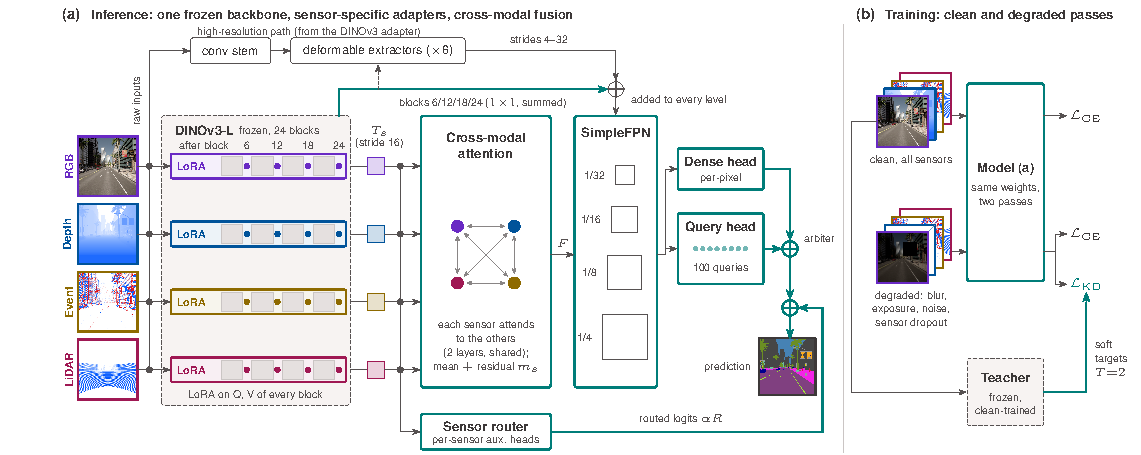
\includegraphics{figures/fig_arch.pdf}
\caption{Network of our model. Each sensor passes through the same frozen DINOv3-L with its own LoRA adapter; the final-block tokens of the sensors are fused by cross-modal attention, while intermediate features of blocks 6, 12, 18, and 24 (all at stride 16) are projected per sensor, summed over sensors, and resampled to the levels of a SimpleFPN that also receives a high-resolution path computed from all sensors. A dense head and a query head are combined by an arbiter; a per-class sensor router, a separate branch on the final-block tokens of each sensor, adds routed logits of per-sensor auxiliary heads to this output. Teal outlines mark the trained components we introduce, grey solid outlines the trained high-resolution path adopted from the DINOv3 adapter, and dashed boxes frozen weights; dots on a line mark where it branches.}
\label{fig:arch}
\end{figure*}
% Facts verified against the code on 2026-10-29: see notes/draft_method_abstract_review_2026-10-29.md §0.

We propose Clean-to-Degraded Two-Pass Distillation (C2D2), a training scheme for multi-sensor segmentation, and apply it to a fusion model built on a frozen vision foundation backbone (Fig.~\ref{fig:arch}); Fig.~\ref{fig:overview} summarizes the training. We also call the resulting model C2D2. We first describe the model (Sections~\ref{sec:m_backbone}--\ref{sec:m_heads}) and then the training scheme (Section~\ref{sec:m_c2d2}).


\subsection{Sensors and Their Failure Modes}\label{sec:m_sensors}
A mobile platform rarely loses all sensors at once; it loses one, partially or completely, under conditions that the other sensors tolerate. An RGB camera gives dense appearance and texture but degrades at night, under low or excessive exposure, and in fog. A depth sensor, or depth reconstructed from stereo or LiDAR, gives geometry that is unaffected by illumination but contains holes on reflective, transparent, and distant surfaces. An event camera reports per-pixel brightness changes with high temporal resolution and dynamic range, but it is silent on static scenes and noisy in low light. A LiDAR gives accurate range on a sparse set of beams that shrinks with distance and is thinned by rain, fog, and absorbing surfaces. Radar, available in one of our benchmarks, measures range and velocity through adverse weather at a very low angular resolution. Each failure is therefore local to one sensor and correlated with a scene condition, which is the situation that a fusion model has to handle without being told which sensor has failed.

\subsection{Frozen Backbone with Sensor-Specific Adapters}\label{sec:m_backbone}
Let $x_s$ denote the input of sensor $s\in\{1,\dots,S\}$, converted to a three-channel image (Section~\ref{sec:exp}). Every $x_s$ is processed by the same DINOv3 ViT-L/16 backbone~\cite{dinov3_2025}, whose weights are frozen. Each sensor has its own low-rank adapters (LoRA)~\cite{lora2022} of rank 8 on the query and value projections of every attention block, so that each sensor can adapt the shared features to its own statistics. The output tokens of the last block form a stride-16 token map $T_s$ per sensor, which is the input of the fusion below. In addition, we take the intermediate features after blocks 6, 12, 18, and 24, which are also stride-16 token maps, project each with a sensor-specific layer normalization and $1\times1$ convolution, and sum the projections over sensors; these four maps are added to the decoder (Section~\ref{sec:m_decoder}).

\subsection{Cross-Modal Fusion}\label{sec:m_fusion}
Each sensor attends to all other sensors. In each of two pre-norm layers, the tokens of sensor $s$ form the queries of a multi-head attention whose keys and values are the input tokens of the other sensors, which stay fixed across the two layers,
\begin{equation}
\hat{T}_s \leftarrow \hat{T}_s + \mathrm{MHA}\big(\hat{T}_s,\ [T_{s'}]_{s'\neq s}\big), \qquad \hat{T}_s^{(0)} = T_s,
\end{equation}
followed by a feed-forward layer. The attention weights are shared across sensors, so every sensor is treated by the same operation. The fused map is the average of the attended maps plus a sensor-specific residual,
\begin{equation}
F = \frac{1}{S}\sum_{s}\hat{T}_s + \sum_{s}\tanh(\gamma_s)\, m_s(T_s),
\end{equation}
where $m_s$ is a small MLP and $\gamma_s$ is a learned scalar per sensor, initialized at 0.1.

\subsection{Sensor Router}\label{sec:m_router}
Each sensor also has an auxiliary head that predicts class logits $A_s$ from $T_s$ and is trained with cross-entropy. A per-class router mixes these predictions pixel by pixel. Its weights are
\begin{equation}
w_{s,k}(p) = \operatorname{softmax}_{s}\big( h_{s,k}(T_s)(p) + \kappa\, r_s(p) \big),
\end{equation}
where $\kappa=1$, $r_s = 1 - H(\sigma(A_s))/\log K$ is the normalized confidence of the auxiliary prediction of sensor $s$ (with gradients stopped), $K$ is the number of classes, and $h_s$ is a small network whose last layer is initialized at zero, so that routing starts from confidence alone. The routed logits $R_k=\sum_s w_{s,k} A_{s,k}$ are added to the final prediction with a learned scale $\alpha$ initialized at zero (Section~\ref{sec:m_heads}). The router is supervised with cross-entropy on $R$ and with a regularizer that favours decisive per-pixel weights. The router thus mixes the sensor-wise auxiliary predictions into the output as a residual; removing it changes accuracy only within the spread between training runs, in opposite directions for two runs (Table~\ref{tab:ablation_loo}).

\subsection{Decoder with a High-Resolution Path}\label{sec:m_decoder}
A SimpleFPN~\cite{vitadapter2023} turns $F$ into a feature pyramid at strides 4, 8, 16, and 32. Because every level is interpolated from stride-16 tokens, structures thinner than a token are poorly represented. We therefore add a high-resolution path that adopts the adapter of the official DINOv3 segmentation code~\cite{dinov3_2025} and extends it to several sensors. As in that adapter, a convolutional stem extracts features at strides 4, 8, 16, and 32 from the raw inputs, deformable-attention extractors, one for each of the four blocks above and two more after the last, let these convolutional features sample semantic evidence from the intermediate features, and, unlike ViT-Adapter~\cite{vitadapter2023}, nothing is injected back into the backbone. Our extension is the handling of several sensors: the stem is shared across sensors and its multi-scale features are projected per sensor and summed, and the intermediate features of all sensors are projected and summed before the extractors sample them. The output of the path is added to the FPN levels, as are the four intermediate features of Section~\ref{sec:m_backbone}, resampled from stride 16 to strides 4, 8, 16, and 32 from the shallowest to the deepest block. Only the high-resolution path carries information finer than a token.

\subsection{Dense and Query Heads}\label{sec:m_heads}
Like CAFuser~\cite{cafuser2025} and DGFusion~\cite{dgfusion2026}, which use a OneFormer-style query head, we combine a dense convolutional head, which gives per-pixel logits $D$ at stride 4, with a Mask2Former-style query head~\cite{mask2former2022} (100 queries, the first $K$ tied to the $K$ classes, six decoder layers over the tokens of all sensors), whose class and mask predictions give per-pixel class scores $Q$. The final logits are
\begin{equation}
\ell_k(p) = D_k(p) + \operatorname{softplus}(\lambda_k)\, Q_k(p) + \alpha\, R_k(p),
\end{equation}
with a learned per-class weight $\lambda_k$. During training, each step uses the dense head, the query head, or both, with probabilities 0.25, 0.25, and 0.5; at inference both are used.

\subsection{Clean-to-Degraded Two-Pass Distillation}\label{sec:m_c2d2}
C2D2 uses every training batch $(x, y)$ twice (Fig.~\ref{fig:overview}).

\emph{Clean pass.} The model sees the clean inputs $x$ and is trained with the segmentation loss $\mathcal{L}_{\mathrm{clean}}$, which combines online hard-example cross-entropy~\cite{ohem2016} on $\ell$ with the losses of the query head, the auxiliary sensor heads, and the router, and two regularizers listed in Section~\ref{sec:exp}.

\emph{Degraded pass.} The model sees a degraded copy $\tilde{x}$. Each sensor of each sample is corrupted independently with probability 0.5. One fifth of the corrupted sensors are removed entirely by setting their normalized input to zero; the others receive one operator drawn from a sensor-specific set: patch dropout and blur for every sensor, a multiplicative gain change for RGB and depth, a colour shift for RGB, holes with a global scale change for depth, dropped and jittered beams for LiDAR, and resolution loss for events. A curriculum moves the degraded input toward the clean one: the input is $x+c\,(\tilde{x}-x)$ with $c$ = 0.3, 0.6, and 1.0 from epochs 0, 10, and 20 onward, while removed sensors stay at zero. Gaussian and salt-and-pepper noise are never used in training, so that the noise evaluation tests corruption that the model has not seen. The degraded pass is supervised by the labels and by a frozen teacher $g$, a model of the same architecture without the high-resolution path that was trained on clean inputs with a longer schedule. The teacher sees the clean input:
\begin{equation}
\mathcal{L}_{\mathrm{deg}} = \mathcal{L}_{\mathrm{ce}}\big(\ell(\tilde{x}), y\big) + \beta\, T^2\, \mathrm{KL}\!\left(\sigma\!\left(\tfrac{g(x)}{T}\right) \Big\|\, \sigma\!\left(\tfrac{\ell(\tilde{x})}{T}\right)\right),
\end{equation}
with $\beta=0.5$ and $T=2$, where $\mathcal{L}_{\mathrm{ce}}$ is the same online hard-example cross-entropy as in the clean pass, $\sigma$ is the softmax over classes and the Kullback--Leibler divergence is averaged over pixels. The total loss is $\mathcal{L}_{\mathrm{clean}} + \mathcal{L}_{\mathrm{deg}}$.

C2D2 needs no condition labels and no degradation labels: the degradation is sampled on the fly, and the teacher only sees clean inputs. It changes training only; the model at inference is the same network run once.

Of these parts, only the degraded pass has a measured effect: removing it leaves clean mIoU within the spread between training runs but lowers the average over the 15 missing-sensor subsets by 9.4 points, consistently in two runs (Table~\ref{tab:ablation_loo}). The contributions of the teacher distillation and of the sensor-specific degradations could not be separated from this spread, and we do not claim either; both are kept in the scheme as used for all reported models \todo{distillation: revisit after DRN-261111-02 (test RMM, NM, val EMM/RMM, clean--degraded agreement, ECE; third L6 seed)}. Distillation from a teacher with complete inputs to a student with missing inputs is also used by~\cite{anyseg2024,rmmss2025}. C2D2 adds no new loss to it; it applies the plain combination of a clean-input teacher and a degraded student to a fusion model on a frozen foundation backbone, where it adds robustness without lowering accuracy when all sensors are present.

\section{Experiments}\label{sec:exp}
\subsection{Implementation Details}
% Source: configs/lecun-deliver_rgbdel_P46_c3only_seed20260821_screen40_A2hires.yaml (TRAIN, OPTIMIZER, SCHEDULER, LOSS, MODEL.M2F, MODEL.P46.C3_PROTO, MODEL.P39).
All sensors are converted to three-channel images as in CMNeXt~\cite{cmnext2023}. We train for 40 epochs with AdamW (learning rate $6\times10^{-4}$, weight decay 0.01), a polynomial schedule with power 0.9, and a 10-epoch warm-up, on $768\times768$ crops with an effective batch size of 16 obtained by gradient accumulation. We use the data augmentation of DGFusion~\cite{dgfusion2026} so that both models see the same augmented images. The clean-pass loss combines online hard-example cross-entropy~\cite{ohem2016} on the final logits with the set-prediction loss of the query head (weight 0.5, with deep supervision), the auxiliary sensor heads (0.5), the router (cross-entropy 0.4 and regularizer 0.01), a class-prototype contrastive term (0.1), and a variance-covariance regularizer on the per-sensor tokens (variance weight 0.1 and covariance weight 0.01, scaled by 1.0 for LiDAR and 0.25 for the other sensors). These terms are inherited from earlier versions of our model; we list them for reproducibility and do not ablate them. The frozen teacher is the same architecture without the high-resolution path, trained for 200 epochs on clean data. All results of our model are the mean of three training runs with different seeds, unless a table states otherwise; the leave-one-out ablation in Table~\ref{tab:ablation_loo} uses one seed.

\subsection{Comparison with Prior Fusion Models}
Table~\ref{tab:deliver} compares \ours{} with fusion models on DELIVER. Part~(a) lists methods with a reported test-split result, which is the split we compare on; part~(b) lists methods that report only validation results, which come from different training and evaluation settings and are shown for completeness. \ours{} reaches 57.74 test mIoU, 1.0 point above the published DGFusion result (56.7). Its margin over MM SAM-adapter, which uses only RGB and depth, is 0.4 points (our three-seed mean). On the validation set, \ours{} scores 70.17 on average, 1.6 points above CAFuser-CAA (68.6); StitchFusion with a Swin-T backbone reports 70.3 without naming the split, so our validation result is not the highest published one. Tables~\ref{tab:muses} and~\ref{tab:mcubes} report the same model on the real MUSES and MCubeS benchmarks \todo{results pending: MUSES four-sensor model, MCubeS transfer}.
% Sources: headline.yaml deliver.ours[0] (57.74 = 3-seed mean; best seed 58.61 is recorded in notes/table_sources.md, not shown: user 2026-11-02). Published DGFusion test = 56.7 (DGFusion Table III p6, notes/sota_survey.md):
%   gap +1.04 (text rounds to 1.0). CAFuser-CAA val 68.6 (CAFuser Table III p6) -> +1.57.
%   68.79 (old draft) has no source and was removed (sota_survey.md 0). StitchFusion Swin-T 70.3: StitchFusion Table 1 p6.
% protocol clusters: repo research/novelty-and-related-work.md l.74-85 (secondary; cite original tables).


% Layout rule (user 2026-10-27): no \resizebox on tables. Every table uses \tabsetup and
% tabular* at \columnwidth, so all tables share one font size and none overflows the column.

% ---------------------------------------------------------------------------
% Table 1. DELIVER, all four sensors.
% Baselines: only the test-unified cluster (DGFusion protocol, "mIoU-test").
%   Do NOT mix with the high cluster (CMNeXt 66.30 / MemorySAM 65.38).
%   Candidate values for todo cells are in repo research/novelty-and-related-work.md:78-83
%   (secondary copy) -> must be taken from each original paper table, cite table+page.
% Ours: experiments/headline.yaml benchmarks.deliver.ours[0] (A2, 3 seeds, legal v2, test@1024).
%   val 3-seed mean 70.17 = tasks/DRN-261019-03 report R03:23.
% ---------------------------------------------------------------------------
\begin{table}[t]
\caption{Comparison with fusion methods on DELIVER (mIoU, \%). Results of other methods are taken from the cited papers.}
\label{tab:deliver}
\centering\tabsetup
\begin{tabular*}{\columnwidth}{@{\extracolsep{\fill}}lllcc@{}}
\toprule
Method & Backbone & Sensors & val & test \\
\midrule
\multicolumn{5}{@{}l}{\emph{(a) All four sensors, test split reported}} \\
CMNeXt~\cite{cmnext2023}$^{a}$ & MiT-B2 & RGB-D-E-L & 66.3 & 53.0 \\
StitchFusion~\cite{stitchfusion2024}$^{a}$ & MiT-B2 & RGB-D-E-L & 68.2 & 53.4 \\
GeminiFusion~\cite{geminifusion2024}$^{a}$ & MiT-B2 & RGB-D-E-L & 66.9 & 54.5 \\
CAFuser-CAA~\cite{cafuser2025} & Swin-T & RGB-D-E-L & 68.6 & 55.2 \\
CAFuser~\cite{cafuser2025} & Swin-T & RGB-D-E-L & 67.8 & 55.6 \\
DGFusion~\cite{dgfusion2026} & Swin-T & RGB-D-E-L & -- & 56.7 \\
\midrule
\multicolumn{5}{@{}l}{\emph{(b) All four sensors, validation split only}} \\
MemorySAM~\cite{memorysam2025}$^{b}$ & Hiera-B+ & RGB-D-E-L & 65.38 & -- \\
MLE-SAM~\cite{mlesam}$^{b}$ & Hiera-B+ & RGB-D-E-L & 64.08 & -- \\
OmniSegmentor~\cite{omnisegmentor2025}$^{b}$ & MiT-B2 & RGB-D-E-L & 67.5 & -- \\
OmniSegmentor~\cite{omnisegmentor2025}$^{b}$ & DFormer-L & RGB-D-E-L & 68.0 & -- \\
HyperDUM~\cite{hyperdum2025} & MiT-B2 & RGB-D-E-L & 67.59 & -- \\
MAGIC~\cite{magic2024} & MiT-B2 & RGB-D-E-L & 67.66 & -- \\
Any2Seg~\cite{any2seg2024} & MiT-B2 & RGB-D-E-L & 68.25 & -- \\
FuseAdapt~\cite{fuseadapt2026}$^{b}$ & DINOv2-B & RGB-D-E-L & 68.33 & -- \\
StitchFusion~\cite{stitchfusion2024}$^{b}$ & Swin-T & RGB-D-E-L & \best{70.3} & -- \\
\midrule
\multicolumn{5}{@{}l}{\emph{(c) Fewer sensors}} \\
MM SAM-adapter~\cite{mmsamadapter2025} & SAM ViT-L & RGB-E & 60.74 & 55.70 \\
MM SAM-adapter~\cite{mmsamadapter2025} & SAM ViT-L & RGB-L & 61.89 & 57.14 \\
MM SAM-adapter~\cite{mmsamadapter2025} & SAM ViT-L & RGB-D & 69.60 & \second{57.35} \\
\midrule
Ours & DINOv3-L & RGB-D-E-L & \second{70.17} & \best{57.74} \\
\bottomrule
\end{tabular*}
\tabnote{$^{a}$Both values as listed by CAFuser~\cite{cafuser2025} (Table~III); the test values were measured by the CAFuser authors. $^{b}$The source does not name the split; listed as validation because it is compared there against validation results. Validation results come from different training and evaluation settings and are not directly comparable. Ours: mean of three seeds.}
\end{table}

% ---------------------------------------------------------------------------
% Table 2. MUSES, four sensors (RGB, event, LiDAR, radar). Only the 4-sensor A2 model
%   (user 2026-09-29; 3-sensor numbers 79.788 etc. are not used).
% Ours: DRN-261019-02 (queued) -> todo. Baselines: headline.yaml benchmarks.muses.
% ---------------------------------------------------------------------------
\begin{table}[t]
\caption{Comparison with fusion methods on MUSES (mIoU, \%). Test results are from the official evaluation server, as reported in the cited papers.}
\label{tab:muses}
\centering\tabsetup
\begin{tabular*}{\columnwidth}{@{\extracolsep{\fill}}lllcc@{}}
\toprule
Method & Backbone & Sensors & val & test \\
\midrule
\multicolumn{5}{@{}l}{\emph{(a) Camera only}~\cite{muses2024}} \\
Mask2Former~\cite{mask2former2022} & Swin-T & RGB & -- & 70.7 \\
SegFormer~\cite{segformer2021} & MiT-B2 & RGB & -- & 72.5 \\
SegFormer~\cite{segformer2021} & MiT-B5 & RGB & -- & 74.7 \\
Mask2Former~\cite{mask2former2022} & Swin-L & RGB & -- & 77.1 \\
\midrule
\multicolumn{5}{@{}l}{\emph{(b) Four sensors}} \\
CMNeXt~\cite{cmnext2023}$^{a}$ & MiT-B2 & RGB-L-R-E & -- & 72.4 \\
GeminiFusion~\cite{geminifusion2024}$^{a}$ & MiT-B2 & RGB-L-R-E & -- & 75.3 \\
CAFuser~\cite{cafuser2025} & Swin-T & RGB-L-R-E & -- & 78.2 \\
CAFuser-CAA~\cite{cafuser2025} & Swin-T & RGB-L-R-E & -- & 78.5 \\
DGFusion~\cite{dgfusion2026} & Swin-T & RGB-L-R-E & -- & 79.5 \\
\midrule
\multicolumn{5}{@{}l}{\emph{(c) Fewer sensors}} \\
FuseAdapt~\cite{fuseadapt2026} & DINOv2-S & RGB-L-E & 77.28 & -- \\
MM SAM-adapter~\cite{mmsamadapter2025} & SAM ViT-L & RGB-E & -- & \second{79.92} \\
MM SAM-adapter~\cite{mmsamadapter2025} & SAM ViT-L & RGB-L & -- & \best{81.07} \\
\midrule
Ours & DINOv3-L & RGB-L-R-E & \td & \td \\
\bottomrule
\end{tabular*}
\tabnote{R: radar. $^{a}$As measured by the CAFuser authors~\cite{cafuser2025} (Table~II).}
\end{table}

% ---------------------------------------------------------------------------
% Table 3. MCubeS (RGB, AoLP, DoLP, NIR). Ours: DRN-261017-02 (A2 transfer, 2 seeds) -> todo.
%   58.07 in headline.yaml is the previous generation (P39.1 recipe), not the paper model.
% ---------------------------------------------------------------------------
\begin{table}[t]
\caption{Comparison on the MCubeS test set with RGB, AoLP, DoLP, and NIR inputs (mIoU, \%).}
\label{tab:mcubes}
\centering\tabsetup
\begin{tabular*}{\columnwidth}{@{\extracolsep{\fill}}lllc@{}}
\toprule
Method & Backbone & Sensors & test \\
\midrule
MCubeSNet~\cite{mcubes2022} & ResNet-101 & RGB-A-D-N & 42.86 \\
ShareCMP~\cite{sharecmp2023} & MiT-B2 & RGB-A-D & 50.99 \\
MLE-SAM~\cite{mlesam} & Hiera-B+ & RGB-A-D-N & 51.02 \\
CMNeXt~\cite{cmnext2023} & MiT-B2 & RGB-A-D-N & 51.54 \\
U3M~\cite{u3m2024} & SegFormer & RGB-A-D-N & 51.69 \\
Any2Seg~\cite{any2seg2024} & MiT-B2 & RGB-A-D-N & 51.91 \\
Cao et al.~\cite{bpcf2026} & MiT-B4 & RGB-A-D-N & 52.22 \\
StitchFusion~\cite{stitchfusion2024} & Swin-T & RGB-A-D-N & 52.3 \\
MemorySAM~\cite{memorysam2025} & Hiera-B+ & RGB-A-D-N & 52.88 \\
MAGIC~\cite{magic2024} & MiT-B2 & RGB-A-D-N & 53.01 \\
MMSFormer~\cite{mmsformer2023} & MiT & RGB-A-D-N & 53.11 \\
StitchFusion~\cite{stitchfusion2024} & MiT-B4 & RGB-A-D-N & 53.92 \\
StitchFusion~\cite{stitchfusion2024} & Swin-L & RGB-A-D-N & \second{55.9} \\
FuseAdapt~\cite{fuseadapt2026} & DINOv2-B & RGB-A-D-N & \best{57.62} \\
\midrule
Ours & DINOv3-L & RGB-A-D-N & \td \\
\bottomrule
\end{tabular*}
\tabnote{A: AoLP, D: DoLP, N: NIR.}
\end{table}

\subsection{Robustness to Missing and Degraded Sensors}
Table~\ref{tab:robust} evaluates robustness with the benchmark of~\cite{mmssbench2025} on the DELIVER validation set. To compare under identical conditions, we run the public evaluation code of the benchmark on our model and on the baselines whose code and weights are public, and list only such methods. \todo{numbers of \ours{} and of the baselines in (b) under the benchmark code (analysis request, 2026-11-04); the earlier measurement with our own scorer (native-resolution labels, no flip) gave EMM 57.85, RMM 61.28--65.53 and NM 58.34/51.92/39.99 and is kept only in the notes until the re-measurement}.
% Sources: tasks/DRN-261019-03/analysis.md (val clean 70.17, EMM15 57.85, RMM 65.53/63.35/61.28); 2503.18445 Tables 3, 7-11;
% drop clean-EMM: ours 70.17-57.85 = 12.32; benchmark models 66.33-37.90 = 28.43 ... 68.20-41.98 = 26.22, MAGIC 66.10-44.97 = 21.13.
% Removed 2026-11-02 (user): test-split S&P-only noise numbers and the DGFusion test EMM sentences (kept in judgment-ledger).
% judgment-ledger:130 DRN-261001-03 (official weights clean 56.73, EMM 31.14, NM drop 52.20 -> 4.53);
% judgment-ledger:117 (reproduction (a) EMM 31.53, NM .20 5.52; retrained (b) EMM 45.52); current.md (4) CAFuser (b) EMM 46.50;
% MAGIC 44.97: arXiv 2503.18445 Table 7 (mIoU_EMM^Avg, MiT-B2, val).

When only one sensor is available (Fig.~\ref{fig:robust}b), the released DGFusion weights collapse to 7.5 mIoU with RGB alone and to 1.1 with event or LiDAR alone, while still reaching 43.3 with depth alone. Training with degraded inputs lifts every single-sensor score, most strongly for RGB (49.0 for the re-trained DGFusion and 53.9 for our model without the high-resolution path).
% Sources: judgment-ledger:130 (official weights single-sensor 7.50/43.33/1.13/1.13); judgment-ledger:117 (retrained 49.0/44.5/25.0/25.0; Q2 3 seeds 53.9/46.0/31.0/22.9).

% ---------------------------------------------------------------------------
% Table 5. Missing and noisy sensors on DELIVER val under the benchmark of arXiv 2503.18445 (user 2026-11-02:
% the paper uses this benchmark; channel-shared salt-and-pepper-only numbers were removed).
% (a) arXiv 2503.18445 (MiT-B2): clean = Table 3 RDEL column; EMM Avg and E(p) = Table 7; RMM Avg r=.75/.5/.25 =
%     Tables 8/9/10; NM Low/Mid/High = Table 11 (mIoU_NM row). Read from the PDF text (notes/missing_bench_survey.md).
% (b) Methods published after the benchmark with the same definition: notes/missing_bench_survey.md (2026-11-02).
%     [removed 2026-11-04, user: open methods only; no public code found] EQUISeg = arXiv 2509.24505 Table 1 p4 (DeLiVER: mIoU 67.90, EMM Avg 48.22, EMM p=0.1 65.75, RMM Avg 50.96,
%     RMM p=0.1 64.64, NM Low 34.87, Mid 19.13); its baseline rows equal 2503.18445 Table 9 (r=0.5) -> RMM column r=.50.
%     RMMSS = 2505.12861 Table 2 p6 (MiT-B0, EMM 49.93, RMM 51.90, r not stated) -> footnote only.
% (c) Baselines measured by us with tools/missing_modality_eval.py on val: analysis inbox 20261102-180010 (pending).
% Fairness check 2026-11-04: benchmark val_mm_NM.py (github Chenfei-Liao/Multi-Modal-Semantic-Segmentation-Robustness-Benchmark)
%   injects S&P (tensor max/min) then Gaussian (RGB, D, L) on the normalized batch from get_val_augmentation; CMNeXt
%   Normalize = ImageNet for img, /255 for others; ours identical (NORM_ALL_MODALS off in configs/eval/a2s821_eval1024_hpca100_probe.yaml).
%   Benchmark NM script evaluates with sliding_predict(flip=True); ours without TTA.
% (d) Ours (A2, 3 seeds): tasks/DRN-261019-03/analysis.md val clean 70.17, EMM15 57.85, RMM r.25/.5/.75
%     65.53/63.35/61.28. NM (DRN-261102-04, nm_mode bench, val) = mean of hpca100 ~/SSDb/jemo_maeng/nmbench_20261102/
%     s821/s902/s903_val/val/missing_modality/summary.json (md5 f98fb583 / 46f6fa86 / 153b8e3b): Low 57.84/59.29/57.88,
%     Mid 51.52/52.79/51.45, High 39.63/40.21/40.12 -> 58.34 / 51.92 / 39.99 (clean in the same files 69.59/71.05/69.86).
%     E(p): inbox 20261102-180010 (seed 903 only so far: 66.10/68.20/69.09).
% ---------------------------------------------------------------------------
\begin{table*}[t]
\caption{Robustness to missing and noisy sensors on the DELIVER validation set under the benchmark protocol of~\cite{mmssbench2025} (mIoU, \%).}
\label{tab:robust}
\centering\tabsetup
\begin{tabular*}{\textwidth}{@{\extracolsep{\fill}}llccccccccccc@{}}
\toprule
 & & & \multicolumn{4}{c}{Entire-missing (EMM)} & \multicolumn{3}{c}{Random-missing (RMM), Avg} & \multicolumn{3}{c}{Noisy (NM)} \\
\cmidrule(lr){4-7}\cmidrule(lr){8-10}\cmidrule(l){11-13}
Method & Backbone & Clean & Avg & E(.20) & E(.10) & E(.05) & $r$=.75 & $r$=.50 & $r$=.25 & Low & Mid & High \\
\midrule
\multicolumn{13}{@{}l}{\emph{(a) Reported by the benchmark~\cite{mmssbench2025}}} \\
CMNeXt~\cite{cmnext2023} & MiT-B2 & 66.33 & 37.90 & 54.46 & 60.41 & 63.38 & 42.17 & 47.49 & \second{53.61} & \best{35.23} & 16.37 & 2.31 \\
GeminiFusion~\cite{geminifusion2024} & MiT-B2 & 66.92 & 37.07 & 54.33 & 60.62 & 63.77 & 39.78 & 42.41 & 49.74 & 5.52 & 4.14 & 3.30 \\
MAGIC~\cite{magic2024} & MiT-B2 & 66.10 & \best{44.97} & \second{58.66} & 62.68 & 64.47 & \second{45.30} & 48.19 & 51.61 & 24.03 & 13.31 & 3.98 \\
MAGIC++~\cite{magicpp2024} & MiT-B2 & \second{67.34} & \second{44.85} & \best{59.18} & \best{63.52} & \second{65.50} & \best{47.06} & \best{49.31} & \best{53.92} & \second{33.12} & \best{18.31} & \second{8.70} \\
StitchFusion~\cite{stitchfusion2024} & MiT-B2 & \best{68.20} & 41.98 & 58.02 & \second{63.29} & \best{65.80} & 45.16 & \second{48.33} & 53.10 & 24.91 & \second{17.11} & \best{9.25} \\
\midrule
\multicolumn{13}{@{}l}{\emph{(b) Evaluated by us with the benchmark code}} \\
DGFusion$^{\ast}$ & Swin-T & \td & \td & \td & \td & \td & \td & \td & \td & \td & \td & \td \\
DGFusion (retrained$^{\dagger}$) & Swin-T & \td & \td & \td & \td & \td & \td & \td & \td & \td & \td & \td \\
CAFuser (retrained$^{\dagger}$) & Swin-T & \td & \td & \td & \td & \td & \td & \td & \td & \td & \td & \td \\
\midrule
Ours & DINOv3-L & \td & \td & \td & \td & \td & \td & \td & \td & \td & \td & \td \\
\bottomrule
\end{tabular*}
\tabnotewide{Avg: mean over the 15 non-empty sensor subsets; E($p$): expectation when each sensor fails independently with probability $p$; RMM $r$: fraction of a removed sensor's values that are zeroed; NM Low/Mid/High: salt-and-pepper density and Gaussian standard deviation (0.05, 0.1), (0.1, 0.2), (0.2, 0.5). All definitions follow~\cite{mmssbench2025} and Section~\ref{sec:sensors}. All entries are produced with the public evaluation code of the benchmark (single forward pass for EMM and RMM, horizontal-flip averaging for NM, labels resized with the input to $1024\times1024$); only methods with public code and weights are listed. $^{\ast}$Released weights. $^{\dagger}$Retrained with synthetic degradation and modality dropout, without distillation. Ours: mean of three seeds; baselines: single runs. Methods that skip a missing input instead of zero-filling it answer a different question and are not listed.}
\end{table*}

% ---------------------------------------------------------------------------
% Fig. robust (data plot). Source numbers and provenance: figures/src/make_data_figs.py (fig_robust).
% ---------------------------------------------------------------------------
\begin{figure}[t]
\centering
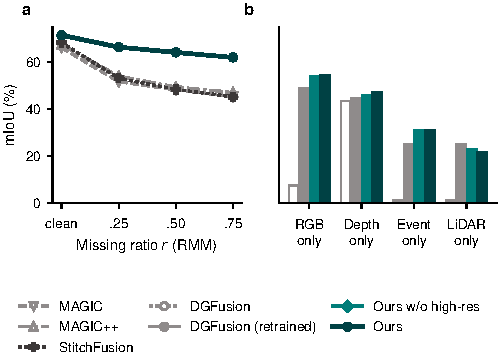
\includegraphics[width=\columnwidth]{figures/fig_robust.pdf}
\caption{Robustness on DELIVER. (a) Random-missing sensors on the validation set: mIoU averaged over the 15 sensor subsets as the missing ratio $r$ grows. Benchmark models (MiT-B2) are taken from~\cite{mmssbench2025}; our curves use our own scorer. (b) A single available sensor on the test set, with the other three zero-filled. Ours: mean of three seeds; baselines: single runs. \todo{(a) our curves: re-measure with the benchmark code; (b) full-model values pending.}}
\label{fig:robust}
\end{figure}

\subsection{Qualitative Results}
Figs.~\ref{fig:failure_scenarios} and~\ref{fig:adverse} show scenes selected by a fixed rule: among all test images, those where the gap between our model and the best of the other models is largest, with no two scenes from the same sequence. With all sensors present (Fig.~\ref{fig:adverse}), this gap is 3.4 to 5.9 points of per-image mIoU on the six scenes shown (2.9 to 5.9 points over the 18 scenes of Appendix~\ref{app:qual}), while the opposite selection, the scene of each condition where another model leads ours the most (Fig.~\ref{fig:reverse}), gives gaps of 8.4 to 10.1 points; per-image differences are therefore modest in both directions when every sensor works \todo{describe the visible error regions; sensor-failure scenes (Fig.~\ref{fig:failure_scenarios}) pending}.

% Fig. sensor-failure scenarios (main qualitative figure). Needs per-image predictions of
% DGFusion (official), DGFusion/CAFuser (retrained) and ours under missing/noisy sensors
% -> analysis request inbox 20261027-182054 item 2.
\begin{figure*}[t]
\centering
\phbox{5.2cm}{Fig.~3 when a sensor fails: rows = depth missing / RGB missing / LiDAR+event missing / RGB with heavy noise; columns = affected input, ground truth, CMNeXt, CAFuser, DGFusion, ours; error pixels in one colour}
\caption{Qualitative comparison on the DELIVER test set when a sensor fails. Rows: depth missing, RGB missing, LiDAR and event missing, and RGB with heavy noise. Columns: affected input, ground truth, CMNeXt, CAFuser, DGFusion, and ours. Each row shows the scene where ours most exceeds the best other method in per-image mIoU, with no repeated sequence.}
\label{fig:failure_scenarios}
\end{figure*}

% Fig. adverse conditions with all sensors present, DELIVER (synthetic) + MUSES (real).
% DELIVER dumps exist: NAS analysis_logs/native_axis_baseline_20261016/{dgfusion,cafuserb}_test1024,
% a2_test1024_dump_20261016/s821 -> analysis request inbox 20261027-182054 item 1. MUSES: item 3.
\begin{figure*}[p]
\centering
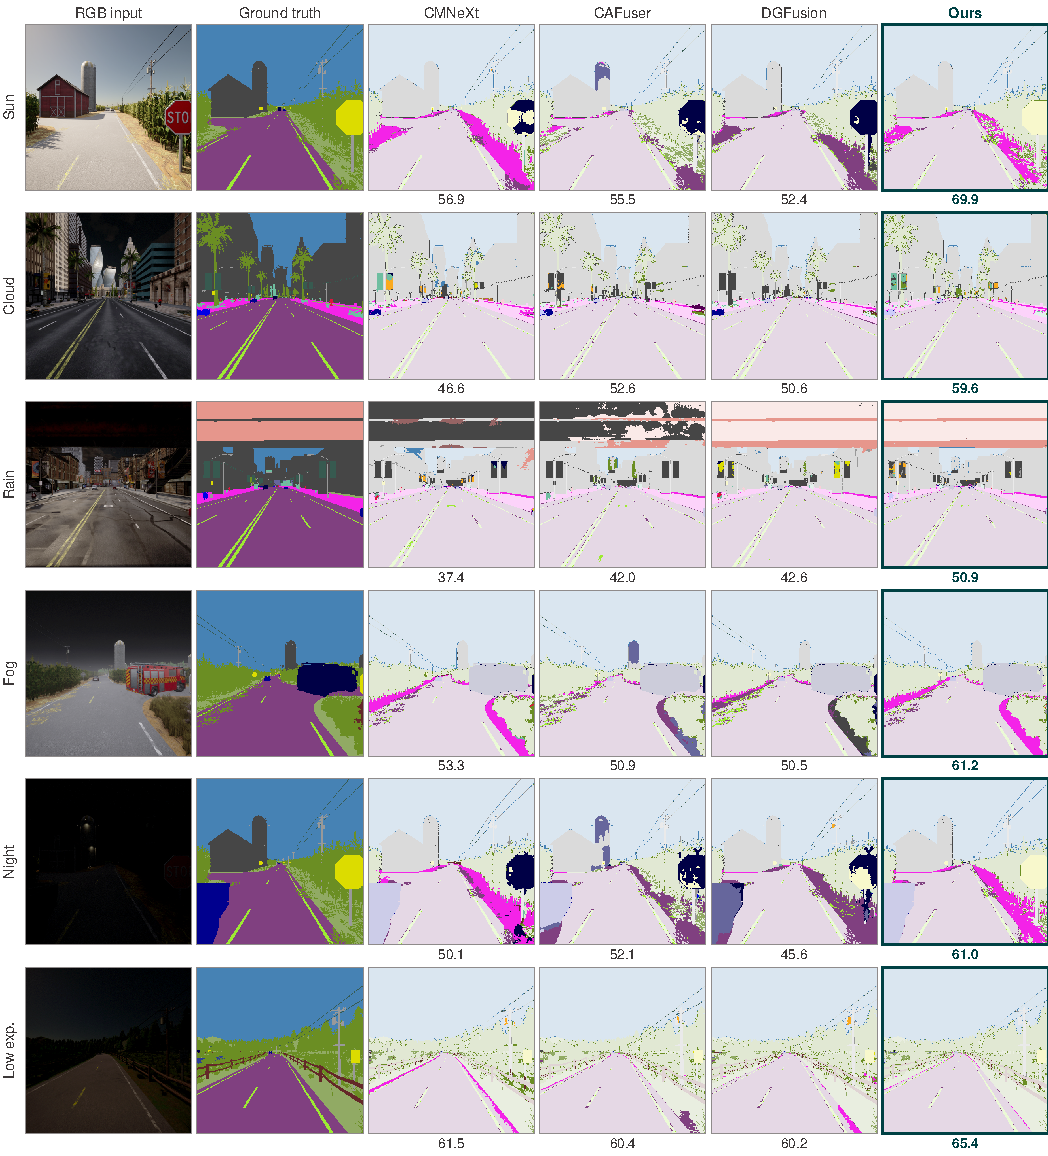
\includegraphics[width=\textwidth]{figures/fig_adverse_deliver.pdf}\\[3pt]
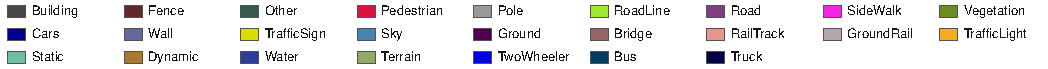
\includegraphics[width=\textwidth]{figures/fig_class_legend_deliver.pdf}
\caption{Qualitative comparison on the DELIVER test set under six conditions with all four sensors. Columns: RGB input, ground truth, CMNeXt, CAFuser, and DGFusion (released weights), and ours. Each row shows the scene where ours most exceeds the best of the other three methods in per-image mIoU, with no two scenes from the same sequence. Faded pixels agree with the ground truth, so colored pixels are errors; numbers give per-image mIoU (\%). More scenes are in Appendix~\ref{app:qual}. \todo{tiles are regenerated when the CMNeXt and CAFuser dumps arrive}}
\label{fig:adverse}
\end{figure*}

% Fig. MUSES real adverse conditions (same layout as fig:adverse; analysis inbox 20261030-122055 P2).
\begin{figure*}[t]
\centering
\phbox{4.6cm}{MUSES val, all sensors: real night / snow / fog / rain; columns = RGB, ground truth, CMNeXt, CAFuser, DGFusion, ours (released weights, release order); same selection rule; waits for the MUSES 4-sensor model}
\caption{\todo{MUSES counterpart of Fig.~\ref{fig:adverse}; same rule on the 250 validation images (test labels are not public)}}
\label{fig:adverse_muses}
\end{figure*}

\subsection{Accuracy per Condition}
Table~\ref{tab:condition} breaks clean test accuracy down by condition \todo{text after the per-condition numbers arrive (analysis request 20261028-183826 item 1)}.

% ---------------------------------------------------------------------------
% Table 5. Clean mIoU per condition on DELIVER test (new 2026-10-28).
% Source: to be computed by analysis from the same dumps as Fig. adverse (inbox addendum).
% ---------------------------------------------------------------------------
\begin{table}[t]
\caption{Per-condition results on the DELIVER test set with all four sensors (mIoU, \%).}
\label{tab:condition}
\centering\tabsetup
\begin{tabular*}{\columnwidth}{@{\extracolsep{\fill}}lccccccc@{}}
\toprule
Model & Sun & Cloud & Rain & Fog & Night & Low exp. & All \\
\midrule
DGFusion$^{\ast}$ & \td & \td & \td & \td & \td & \td & \second{56.73} \\
DGFusion (retrained$^{\dagger}$) & \td & \td & \td & \td & \td & \td & 54.77 \\
CAFuser (retrained$^{\dagger}$) & \td & \td & \td & \td & \td & \td & 55.79 \\
Ours & \td & \td & \td & \td & \td & \td & \best{57.74} \\
\bottomrule
\end{tabular*}
\tabnote{$^{\ast}$Released weights. $^{\dagger}$Retrained with synthetic degradation and modality dropout, without distillation. All: test mIoU over all conditions from the same measurement as the other columns.}
\end{table}

\subsection{Ablation}
Table~\ref{tab:abl_robust} measures the two additions, the C2D2 training scheme and the high-resolution path, over three seeds, and Table~\ref{tab:ablation_loo} removes one component at a time from the full model with one seed. A frozen DINOv3-L with LoRA on RGB alone already reaches 55.14 mIoU on the test set (one seed), within 1.6 points of DGFusion with four sensors, so a large part of the accuracy comes from the foundation model. On the test set, the high-resolution path raises mIoU from 56.59 to 57.74 \todo{effect of C2D2 alone: three-seed test mean of the clean-trained model}. Removing cross-modal attention costs 0.85 points. \todo{the degradation-pass and distillation rows (L5, L6) pending}.
% Sources: judgment-ledger 2026-10-28 rows DRN-261020-08/-09/-10/-12 (seed 821, legal v2 test@1024);
% E1 screen s821 55.94: status/current.md (4); Q2/A2 s821 57.73/58.61: tasks/DRN-261019-03/analysis.md.

% ---------------------------------------------------------------------------
% Table 6. Ablation on DELIVER test, seed 821, 40 epochs, legal v2.
% RGB-only 55.14 = judgment-ledger 2026-10-28 DRN-261020-08 (adopted as ladder row).
% L2 mean fusion 57.76 = judgment-ledger 2026-10-28 (L4 dense head only 57.89 removed from the paper: user 2026-11-04, query-head ablation dropped)
%   rows DRN-261020-09/-10/-12 (test@1024 legal v2, seed 821). L2 also removes the trunk expansion
%   (code constraint, ledger note). L5 DRN-261020-13 / L6 -14 evaluating; mean-fusion ladder -07 running.
% mean fusion = DRN-261020-07 (evaluating). E1 screen s821 55.94 = status/current.md (4).
% Q2 s821 57.73 / EMM 48.68 and A2 s821 58.61 / EMM 49.12 = tasks/DRN-261019-03/analysis.md.
% Leave-one-out: L2 DRN-261020-10, L4 -12, L5 -13, L6 -14, L7 DRN-261029-01. L3 withdrawn. L1 (one adapter for all sensors) is
% excluded from this paper (user 2026-11-02, inbox 20261102-191138) and kept for the separate RA-L paper.
% ---------------------------------------------------------------------------
% Table "incremental ablation" (tab:ablation) removed 2026-11-04 (user): its C2D2 / high-res rows duplicated tab:abl_robust.

% Table 6b. Leave one component out of the full model (one seed, 40 epochs). Sources as Table 6 comment above;
% L5 DRN-261020-13 (evaluating), L6 -14 (judging), L7 DRN-261029-01 (running) -> todo until verdicts.
\begin{table}[t]
\caption{Leave-one-out ablation on the DELIVER test set (mIoU, \%). Each row removes one component from the full model (last row).}
\label{tab:ablation_loo}
\centering\tabsetup
\begin{tabular*}{\columnwidth}{@{\extracolsep{\fill}}cccccc@{}}
\toprule
Cross- & Degr. & Phys. & Teacher & Clean & EMM \\
modal & pass & degr. & KD & & \\
\midrule
\cmark & \xmark & \xmark & \cmark & \td & \td \\
\cmark & \cmark & \cmark & \xmark & \td & \td \\
\cmark & \cmark & \xmark & \cmark & \td & \td \\
\xmark$^{*}$ & \cmark & \cmark & \cmark & \second{57.76} & \td \\
\cmark & \cmark & \cmark & \cmark & \best{58.61} & 49.12 \\
\bottomrule
\end{tabular*}
\tabnote{All rows keep the high-resolution path. Degr.\ pass: the second, degraded forward pass of the C2D2 scheme. Phys.\ degr.: sensor-specific degradations (blur, exposure, depth holes, beam drop, event down-sampling) instead of zero-filling only, with the same missing-sensor rate. Teacher KD: the distillation term on the degraded pass. $^{*}$Token averaging; also removes the sensor-specific residual $m_s$ of Eq.~(2).}
\end{table}

% Table 6c. Robustness ablation, 3 seeds, DELIVER val, benchmark protocol (user 2026-11-02).
% w/o high-res = Q2 3 seeds val: tasks/DRN-261019-03/analysis.md (clean 67.91, EMM15 56.87, RMM .25/.5/.75 64.08/62.46/60.69).
% w/o C2D2 and high-res (E1 40ep) val: analysis inbox 20261102-180010 (pending).
% w/o C2D2 and high-res = E1 40-ep screen 3 seeds, EMM 40.01 (judgment-ledger 2026-10-01 row);
% w/o high-res = Q2 3 seeds, full = A2 3 seeds: tasks/DRN-261019-03/analysis.md (moved from Table robust (b)).
% MCubeS rows: DRN-261031-01 (w/o C2D2, legal eval pending) and DRN-261017-02 (C2D2, training).
\begin{table}[t]
\caption{Effect of the C2D2 training scheme and the high-resolution path on accuracy and robustness (mIoU, \%, mean of three seeds).}
\label{tab:abl_robust}
\centering\tabsetup
\begin{tabular*}{\columnwidth}{@{\extracolsep{\fill}}cccccccc@{}}
\toprule
C2D2 & High- & Test & \multicolumn{5}{c}{Validation} \\
\cmidrule(l){4-8}
tr. & res & Clean & Clean & EMM & RMM .75 & .50 & .25 \\
\midrule
\multicolumn{8}{@{}l}{\emph{(a) DELIVER, mean of 3 seeds}} \\
\xmark & \xmark & \td & \td & \td & \td & \td & \td \\
\cmark & \xmark & \second{56.59} & \second{67.91} & \second{56.87} & \second{60.69} & \second{62.46} & \second{64.08} \\
\cmark & \cmark & \best{57.74} & \best{70.17} & \best{57.85} & \best{61.28} & \best{63.35} & \best{65.53} \\
\midrule
\multicolumn{8}{@{}l}{\emph{(b) MCubeS}} \\
\xmark & \cmark & \td & & & & & \\
\cmark & \cmark & \td & & & & & \\
\bottomrule
\end{tabular*}
\tabnote{C2D2 tr.: trained with the C2D2 scheme (clean pass, degraded pass, and teacher distillation). Test: test-set mIoU with all sensors. The validation columns of (a) use our own scorer (native-resolution labels, no flip) until the re-measurement with the benchmark code of Table~\ref{tab:robust}; EMM and RMM are averages over the 15 sensor subsets.}
\end{table}

\subsection{Computational Cost}
The C2D2 training scheme changes only how the model is trained: the second, degraded pass and the frozen teacher are used during training and removed afterwards, so the deployed model is the same network with or without this scheme. Its cost therefore comes from the architecture, which Table~\ref{tab:cost} reports at inference. The backbone is frozen, and our model has about as many trainable parameters as the baselines (74.0M against 75.0M and 78.9M). Because every sensor passes through the frozen ViT-L, however, it needs 14.6 times the operations and 2.9 times the latency of DGFusion, about four images per second for four sensors at $1024\times1024$ on one RTX 4090. The high-resolution path adds 15.2M parameters, about 2\% of the operations, and 13\% of the latency. \todo{add the DINOv3-B operating point (DRN-261102-01/-02) to show the accuracy--cost trade-off of a smaller backbone}
% Source: .claude_logs/tasks/DRN-261027-02/analysis.md table (l.14-19), verdict adopt 2026-11-03; raw NAS analysis_logs/cost_table_20261104{,b,c}/.
% Ratios: 10135/695.6 = 14.57; 254.5/88.9 = 2.86; high-res = A2 - Q2: 377.05-361.87 = 15.18M, (10135-9922)/9922 = 2.1%, 254.5/224.8 = 1.13.

% ---------------------------------------------------------------------------
% Table 7. Cost on DELIVER at 1024, same GPU. DRN-261027-02 (adopted; notes/table_sources.md cost rows).
% ---------------------------------------------------------------------------
\begin{table}[t]
\caption{Inference cost on DELIVER with four sensors ($1024\times1024$ input, batch size 1, one RTX 4090, bf16). Trainable: parameters updated during training. The C2D2 training scheme adds no inference cost.}
\label{tab:cost}
\centering\tabsetup
\begin{tabular*}{\columnwidth}{@{\extracolsep{\fill}}lccccc@{}}
\toprule
Model & Params & Trainable & GFLOPs & Latency & Memory \\
 & (M) & (M) & & (ms) & (GB) \\
\midrule
DGFusion~\cite{dgfusion2026} & 78.88 & 78.88 & 695.6 & 88.9 & 1.83 \\
CAFuser~\cite{cafuser2025} & 75.01 & 75.01 & 670.8 & 83.1 & 1.57 \\
Ours & 377.05 & 73.98 & 10{,}135 & 254.5 & 2.47 \\
\bottomrule
\end{tabular*}
\end{table}

\section{Analysis}\label{sec:analysis}

% Figure plan: notes/figure_guide.md §2. Qualitative scenes come from recorded dumps only
% (path + md5 in the figure source note) and the selection rule is stated in the caption.

\subsection{Where Sensor Over-Reliance Comes From}
A fusion model can lean on one sensor because its architecture or supervision favours that sensor, or because the training data make that sensor sufficient. DGFusion~\cite{dgfusion2026} is a useful test case: it adds depth supervision to its fusion, and removing depth costs our reproduction of DGFusion 23 to 37 points depending on the condition (Fig.~\ref{fig:dependence}). If the depth supervision caused this dependence, a model without it should behave differently.

Our model trained on clean inputs, which has no depth supervision, also depends on depth: removing it costs 14.3 to 14.8 points in sun, cloud, rain, and fog, 17.9 at night, and 25.0 at low exposure, less than for DGFusion but growing towards the dark conditions in the same way. Our full model, trained with the C2D2 scheme, loses only 0.6 to 1.5 points in sun, cloud, rain, and fog, 4.3 at night, and 9.6 at low exposure (all on the test split; three seeds for the full model, two for the clean-trained one). The effect also appears in a second architecture: when we re-train DGFusion with the same synthetic degradation, removing depth entirely costs 4.7 points, whereas it costs 33.3 points for our reproduction trained without degradation and 33.4 for the released weights (test split, our evaluation code; \todo{re-measure with the benchmark code of Table~\ref{tab:robust}}).
% Sources: ours = figures/source_data/fig_dependence.csv (2026-11-09, R1 depth0 dumps vs clean dumps, test); DGFusion reproduction (a) = judgment-ledger:112;
% judgment-ledger:117 (reproduction (a) -> retrained (b): depth fully missing -33.3 -> -4.7); judgment-ledger:130 (official weights -33.4).

These measurements suggest that, on DELIVER, the dependence on depth comes mainly from training without degraded sensors rather than from a particular fusion design or supervision \todo{final wording after FU-04 (C2D2 applied to DGFusion and CAFuser)}. A plausible reason is that DELIVER renders depth without noise or holes, so training on complete inputs finds a shortcut that real depth sensors would not offer. The comparison has one caveat: our two curves differ in training and also in the high-resolution path, which only the full model has; an earlier measurement on the validation split of the C2D2-trained model without the path (3.4 to 13.4 points) indicates that most of the reduction comes from the training.

\begin{figure}[t]
\centering
% Source numbers and provenance: figures/src/make_data_figs.py (fig_dependence). Full table: sections/supp_tables.tex (Table S1).
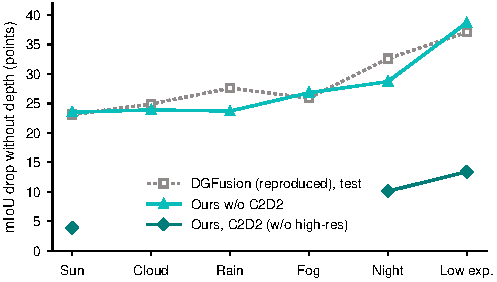
\includegraphics[width=\columnwidth]{figures/fig_dependence.pdf}
\caption{Dependence on depth across conditions on the DELIVER test set: change in mIoU when the depth input is zero-filled at inference (closer to zero means less dependence). Ours w/o C2D2: clean training, without the high-resolution path (mean of two seeds); Ours: full model (mean of three seeds).}
\label{fig:dependence}
\end{figure}

\subsection{What the High-Resolution Path Adds}
The high-resolution path raises clean test mIoU by 1.15 points on average over three seeds (from 56.59 to 57.74 on the test split). Fig.~\ref{fig:thin} shows where the gain comes from. Averaged over the three seeds, Static gains 10.4 points, Pedestrian 3.8, TrafficSign 3.1, and Pole 2.1, and the four thin classes gain 3.0 points together (Table~\ref{tab:thin}). Table~\ref{tab:thin} compares every class with the released baselines. Our model is ahead of all three on 16 of the 25 classes, and on 15 of them every one of its three seeds is ahead. The largest margins are on Wall (+11.3 points), TrafficSign (+8.0), Water (+6.8), Truck (+5.5), and Static (+5.4). On Wall, TrafficSign, Truck, Water, Building, and Dynamic, the model without the path is already ahead of every baseline in all three seeds, by 9.2, 4.9, 4.4, 2.8, 1.8, and 1.2 points; Appendix~\ref{app:ladder} splits these margins over the stages of the model. On Static, SideWalk, Cars, and GroundRail, the model without the path is behind the best baseline in every seed, and the path turns this into a lead; on Static it adds 10.4 points. This matches what the path changes in the architecture: it computes features at stride 4 from the raw pixels, whereas every other input of the decoder is interpolated from stride-16 tokens (Section~\ref{sec:m_decoder}). Measured on the test set, the magnitude of its stride-4 features is 2.5 times higher on pixels of the four thin classes than on average over the image, against 0.93 for the tapped backbone features at the same level, and switching the path off at inference, a configuration not seen in training, costs the thin classes 2.2 times as much IoU as the other classes \todo{feature-magnitude figure from NAS analysis\_logs/hires\_viz\_a2s821\_20261104 after the verdict of DRN-261104-02; per-class split of the shared part needs the clean-trained and RGB-only models}. The baselines stay ahead on RailTrack, where DGFusion reaches 64.5 and our seeds vary between 26 and 57, and on the thin vertical classes TrafficLight, Pole, and Pedestrian, where CAFuser is best; the high-resolution path narrows the gap on Pole and Pedestrian but does not close it, and it widens the gap on TrafficLight (Section~\ref{sec:failure_tl}). Appendix~\ref{app:ladder} traces both losses to the stage where they appear. The gain comes mainly from recall: for Pole the recall rises from 0.75 to 0.78 and for Pedestrian from 0.89 to 0.90 \todo{confirm these recall values (two seeds, NAS analysis\_logs/a2\_thin\_anatomy\_20261018/summary.md) through the analysis session before citing}. Two classes lose: TrafficLight by 4.1 points and RailTrack by 7.2. RailTrack varies strongly between seeds even without the path (58.5, 32.6, and 45.1 for the three seeds), so we do not interpret its change. The TrafficLight loss, in contrast, is systematic and is analysed next.
% Sources: per-class 3-seed CSV .claude_logs/experiments/analysis/DRN-261018-01/a2_vs_q2_perclass_3seed.csv (d_mean3 column);
% thin-4 mean +3.04 and 24-class Δ +1.50: tasks/DRN-261018-01/analysis.md.

\begin{figure}[t]
\centering
% Source: .claude_logs/experiments/analysis/DRN-261018-01/a2_vs_q2_perclass_3seed.csv (3 seeds, legal v2 test 1024);
% plot: figures/src/make_data_figs.py (fig_thin).
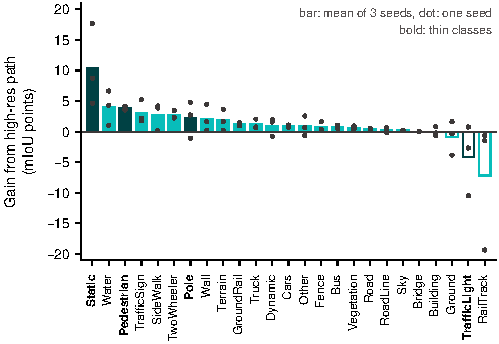
\includegraphics[width=\columnwidth]{figures/fig_thin.pdf}
\caption{Per-class IoU gain from the high-resolution path on the DELIVER test set (full model minus the same model without the path). Bars: mean of three seeds; dots: individual seeds. \todo{add zoomed crops of thin objects (Q2 dumps on yeon).}}
\label{fig:thin}
\end{figure}

% Table perclass (user 2026-11-09): all 25 classes, DELIVER test, legal v2 axis.
% Baselines: NAS analysis_logs/baseline_official_dump_20261104/class_iou_official.csv (released weights, 1024 prediction -> native GT nearest).
% Ours: .claude_logs/experiments/analysis/DRN-261018-01/a2_vs_q2_perclass_3seed.csv (a2* = Ours, q2* = w/o high-res), 3-seed means.
% Rows sorted by Delta = Ours - best released baseline; bold/underline = best/second in the row (hand-marked, not mark_best.py).
\begin{table}[t]
\caption{Per-class IoU on the DELIVER test set (\%), sorted by the margin of ours over the best released baseline (last column).}
\label{tab:thin}
\centering\tabsetup
\begin{tabular*}{\columnwidth}{@{\extracolsep{\fill}}lcccccc@{}}
\toprule
Class & CMNeXt$^{\ast}$ & CAFuser$^{\ast}$ & DGFusion$^{\ast}$ & Ours w/o & Ours & $\Delta$ \\
 & & & & high-res & & \\
\midrule
\multicolumn{7}{@{}l}{\emph{(a) Ours ahead of every released baseline (16 classes)}} \\
Wall & 3.72 & 2.82 & 4.03 & \second{13.20} & \best{15.31} & +11.28 \\
TrafficSign & 38.37 & 45.57 & 45.14 & \second{50.46} & \best{53.54} & +7.97 \\
Water & 2.02 & 0.17 & 0.00 & \second{4.79} & \best{8.80} & +6.77 \\
Truck & 77.43 & 89.35 & 89.15 & \second{93.73} & \best{94.90} & +5.54 \\
Static & 31.26 & 33.91 & \second{38.36} & 33.36 & \best{43.71} & +5.36 \\
TwoWheeler & 61.83 & 68.95 & 65.96 & \second{69.02} & \best{71.69} & +2.75 \\
Dynamic & 6.78 & 7.28 & 8.55 & \second{9.77} & \best{10.69} & +2.14 \\
Terrain & 59.75 & 68.96 & 63.59 & \second{69.05} & \best{70.89} & +1.94 \\
Building & 87.45 & 86.89 & 87.55 & \best{89.36} & \second{89.34} & +1.79 \\
Road & 96.47 & 96.67 & 96.52 & \second{97.21} & \best{97.67} & +0.99 \\
RoadLine & 81.42 & 77.08 & 77.50 & \second{82.06} & \best{82.36} & +0.94 \\
GroundRail & 77.23 & 79.56 & \second{80.59} & 80.23 & \best{81.49} & +0.90 \\
Bus & 94.34 & 93.69 & 94.18 & \second{94.35} & \best{95.08} & +0.75 \\
Vegetation & 82.46 & 83.75 & 83.56 & \second{83.86} & \best{84.49} & +0.74 \\
SideWalk$^{\S}$ & 67.64 & \second{78.49} & 78.06 & 76.11 & \best{78.85} & +0.36 \\
Cars & 93.74 & 94.40 & \second{94.61} & 93.89 & \best{94.80} & +0.19 \\
\midrule
\multicolumn{7}{@{}l}{\emph{(b) A released baseline ahead (9 classes)}} \\
Bridge & \best{0.03} & 0.00 & 0.00 & \second{0.02} & 0.01 & $-$0.02 \\
Sky & 97.15 & \best{98.20} & 97.99 & 97.97 & \second{98.15} & $-$0.05 \\
Ground & 4.38 & 5.68 & \second{7.24} & \best{7.64} & 6.78 & $-$0.46 \\
Pedestrian & 76.64 & \second{82.93} & \best{83.06} & 76.94 & 80.74 & $-$2.31 \\
Fence & 48.04 & \second{52.59} & \best{53.59} & 49.69 & 50.46 & $-$3.13 \\
Other & 5.76 & \best{7.65} & \second{7.22} & 3.11 & 3.99 & $-$3.67 \\
Pole & 48.39 & \best{60.64} & \second{55.65} & 51.94 & 54.08 & $-$6.56 \\
TrafficLight & 31.96 & \best{46.21} & 41.14 & \second{41.67} & 37.52 & $-$8.68 \\
RailTrack & 34.22 & 33.00 & \best{64.46} & \second{45.41} & 38.25 & $-$26.21 \\
\midrule
mIoU & 52.34 & 55.78 & 56.71 & 56.59 & 57.74 & +1.04 \\
\bottomrule
\end{tabular*}
\tabnote{$^{\ast}$Released weights, evaluated with our code because the papers do not report per-class IoU. Ours: mean of three seeds; in (a), every seed of ours is ahead of the best baseline except where marked $^{\S}$. Bold: best in the row; underline: second.}
\end{table}

\subsection{Failure Case: Posters Read as Traffic Lights}\label{sec:failure_tl}
With the high-resolution path, the recall of TrafficLight rises (0.80 to 0.85) but its precision falls (0.46 to 0.41) \todo{same confirmation as above}. Fig.~\ref{fig:failure} shows where the extra false positives appear. In the scenes with the largest increase, billboards and posters, labelled as \emph{Other}, are painted as traffic lights, and in one rainy scene a traffic sign is. The two classes share fine structure, a small bright rectangular shape on a pole or a wall, but differ in context. Because the high-resolution features are added to every pyramid level without a gate, fine detail reaches the dense per-pixel classifier directly, and the classifier can follow the detail without enough context. This mechanism is a hypothesis that our measurements are consistent with but do not prove; we discuss a remedy in Section~\ref{sec:conclusion}.
% Source: NAS analysis_logs/a2_tl_fp_scenes_20261022/README.md (4 scenes; A2 vs Q2 TrafficLight FP pixels
% 15258 vs 3620, 13705 vs 3752, 10304 vs 2008, 12229 vs 9008; selection rule: top-20 by A2 FP - Q2 FP, no repeated condition).

\begin{figure}[t]
\centering
% Assets: NAS analysis_logs/a2_tl_fp_scenes_20261022 (4 scenes, README.md has the selection rule).
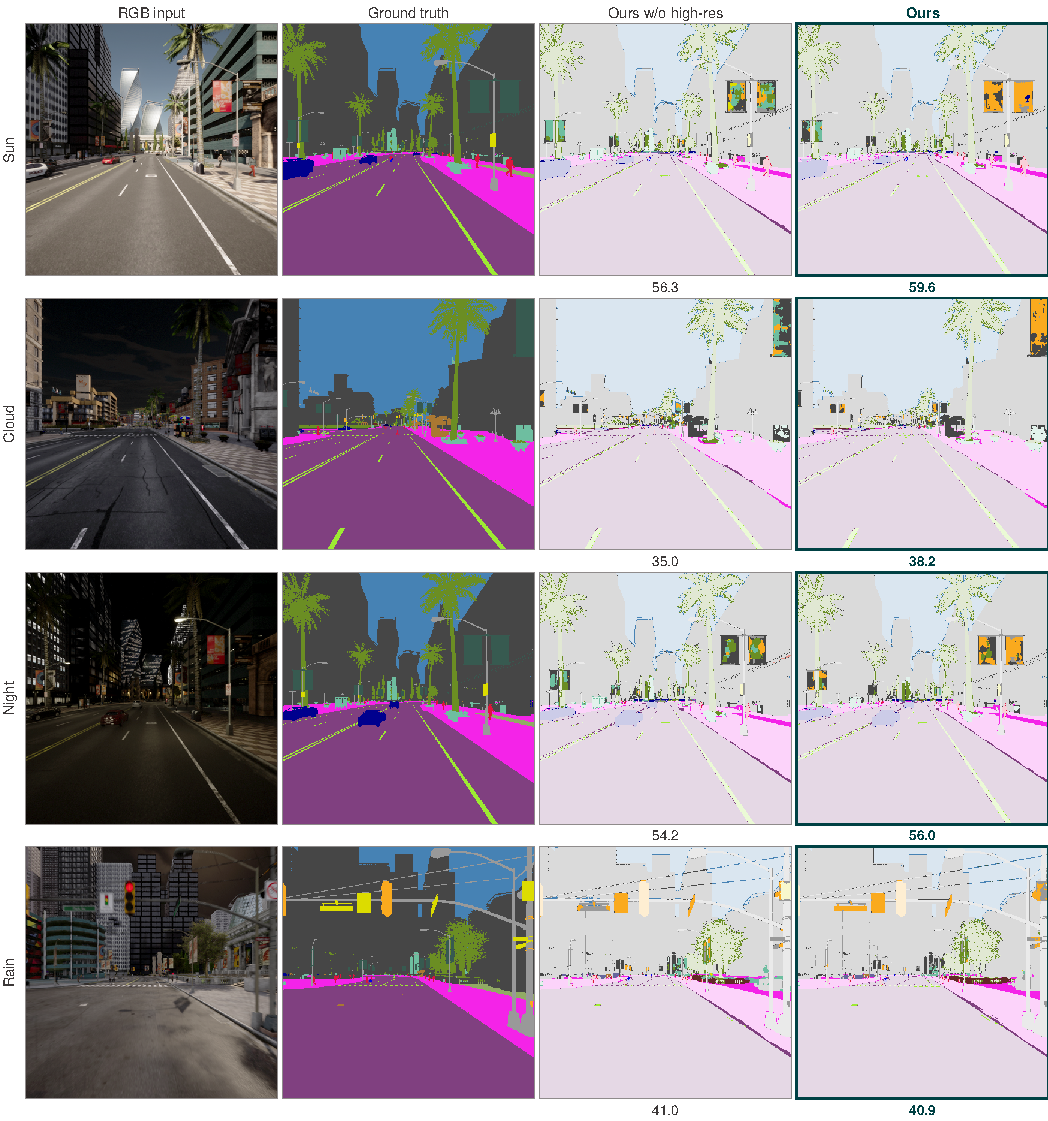
\includegraphics[width=\columnwidth]{figures/fig_tl_deliver.pdf}
\caption{Failure case of the high-resolution path on the DELIVER test set: posters and signs predicted as traffic lights. Scenes are drawn from the 20 test images where the path adds the most TrafficLight false positives, one per condition. Columns: RGB input, ground truth, our model without and with the path (seed 821 pair). Faded pixels agree with the ground truth; numbers give per-image mIoU (\%); colours follow the key of Fig.~\ref{fig:adverse}.}
\label{fig:failure}
\end{figure}

\subsection{Scenes Where a Baseline Is Better}
Fig.~\ref{fig:reverse} applies the selection rule of Fig.~\ref{fig:adverse} in the opposite direction: for each condition it shows the test scene where another model leads ours by the largest per-image mIoU. In four of the six conditions that model is DGFusion and in two it is CAFuser, and the gap is 8.5 to 12.9 points, similar in size to the largest gaps in our favour (3.9 to 13.0 points in Fig.~\ref{fig:adverse}). These scenes are not chosen to be typical; they bound how much a single image can favour a baseline when all sensors are present \todo{describe the error regions once read; check whether the losses share a class (e.g., sidewalk, vegetation boundaries)}.

\begin{figure*}[p]
\centering
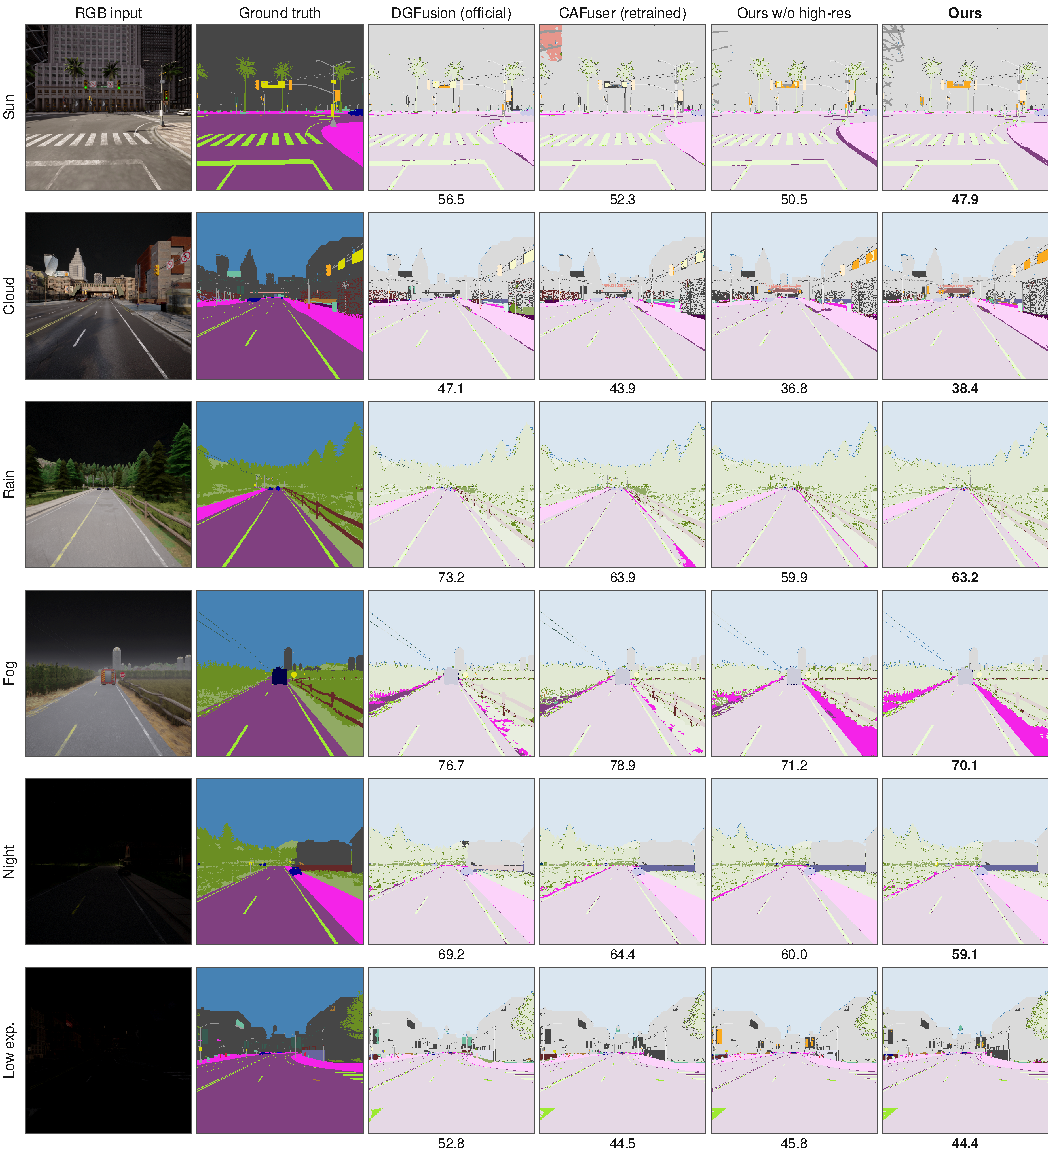
\includegraphics[width=\textwidth]{figures/fig_reverse_deliver.pdf}\\[3pt]
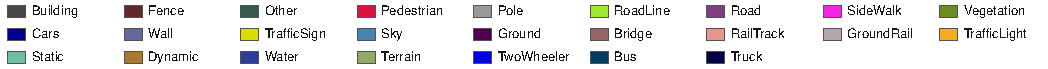
\includegraphics[width=\textwidth]{figures/fig_class_legend_deliver.pdf}
\caption{Failure cases on the DELIVER test set with all four sensors. Each row shows the scene where the best of the other three methods most exceeds ours in per-image mIoU, with no two scenes from the same sequence. Display as in Fig.~\ref{fig:adverse}.}
\label{fig:reverse}
\end{figure*}

\subsection{Limitations}
First, DELIVER is synthetic, and its complete depth is the reason the shortcut exists; the size of the effect on real depth sensors remains to be measured, and MUSES does not contain depth. Second, our main runs use a 40-epoch schedule and three seeds, the ablations one seed, and the baselines are single runs, so differences below about one point should not be over-read. Third, whether the high-resolution path, whose convolutional stem sees raw pixels, changes robustness to pixel noise has not been measured: under the benchmark noise our model keeps 58.63, 52.00, and 39.87 mIoU at the three levels (Table~\ref{tab:robust}), but the same measurement without the path is missing. Fourth, the frozen ViT-L processes every sensor separately, so inference costs 14.6 times the operations and 2.9 times the latency of DGFusion (Table~\ref{tab:cost}); sharing tokens across sensors or a smaller backbone would reduce this, which we have not evaluated.

\section{Conclusion}\label{sec:conclusion}
We proposed C2D2, a two-pass training scheme that adds a synthetically degraded pass, distilled from a frozen clean-input teacher, to ordinary training. Applied to a fusion model on a frozen DINOv3 backbone with sensor-specific adapters, cross-modal attention, and a high-resolution path, it gives the highest test mIoU among published four-sensor fusion models on DELIVER while keeping the model robust when sensors are removed or corrupted, and it reaches 80.01 mIoU on the MUSES test server and 59.78 on MCubeS, above the best published four-sensor and overall results, respectively. Our analysis indicates that the heavy dependence of fusion models on depth in DELIVER comes mainly from training without degraded sensors \todo{wording after FU-04 and FU-05}. It also exposes what remains: the high-resolution path recovers thin objects but lets fine detail mislead the per-pixel classifier, as in posters read as traffic lights, which suggests routing fine detail to mask prediction rather than to per-pixel classification. Measuring the same dependence on real depth sensors is the next step that our synthetic-data findings call for.

\clearpage % flush the main-text figures before the appendix (user 2026-11-02: no page limit)
% Appendix: additional qualitative results (user 2026-11-02: no page limit, up to ~18 pages).
% Figures: figures/src/make_qual_figs.py (scenes chosen in figures/qualbank/selection.yaml from
% figures/source_data/qualbank/deliver_candidates.csv, built over all 1897 test images by figures/qualbank/qualbank.py)
\appendices
\section{Additional Qualitative Results}
\label{app:qual}
Figs.~\ref{fig:supp1}--\ref{fig:supp3} show the second- and third-ranked scenes of every condition under the rule of Fig.~\ref{fig:adverse} (largest per-image mIoU gap between our model and the best of the other three models; no two scenes of a condition from the same sequence). Together with Fig.~\ref{fig:adverse} they are the 18 highest-ranked scenes of the five weather and lighting conditions and under-exposure. The candidates are computed over all 1897 test images of every model, so any scene can be replaced without new inference.

The rule picks scenes in our favour by construction. To show what an ordinary scene looks like, Fig.~\ref{fig:typical} takes, for each condition, the scene whose gap is closest to that condition's median gap. Note that the median gap is slightly negative (about $-1$ to $-2$ points in every condition): the reference is, per image, the best of three other models, so a single model rarely beats it on a typical image even when it has the highest dataset mIoU.

The DELIVER test split also contains sequences with a built-in sensor fault (over-exposure, motion blur, LiDAR jitter, low-resolution events). Figs.~\ref{fig:cases} and~\ref{fig:cases_reverse} show the scene of each fault with the largest gap in our favour and against us; the second column is the affected sensor. Fig.~\ref{fig:thin_scenes} ranks scenes by the gain on one thin class instead of the image mIoU. \todo{MUSES and MCubeS scenes; DELIVER missing-sensor scenes}

\begin{figure*}[p]
\centering
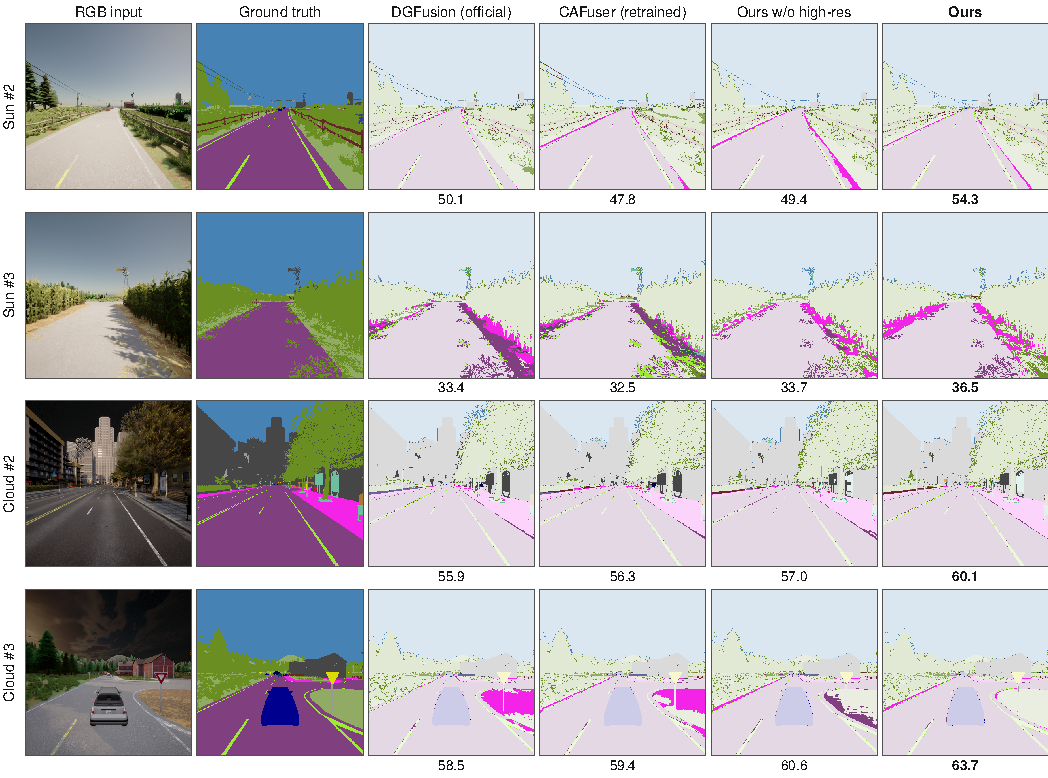
\includegraphics[width=\textwidth]{figures/fig_supp_deliver_1.pdf}\\[3pt]
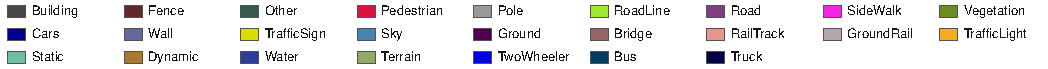
\includegraphics[width=\textwidth]{figures/fig_class_legend_deliver.pdf}
\caption{Additional qualitative results on the DELIVER test set for sun and cloud: the second- and third-ranked scenes under the selection rule of Fig.~\ref{fig:adverse}. Faded pixels agree with the ground truth; numbers give per-image mIoU (\%).}
\label{fig:supp1}
\end{figure*}

\begin{figure*}[p]
\centering
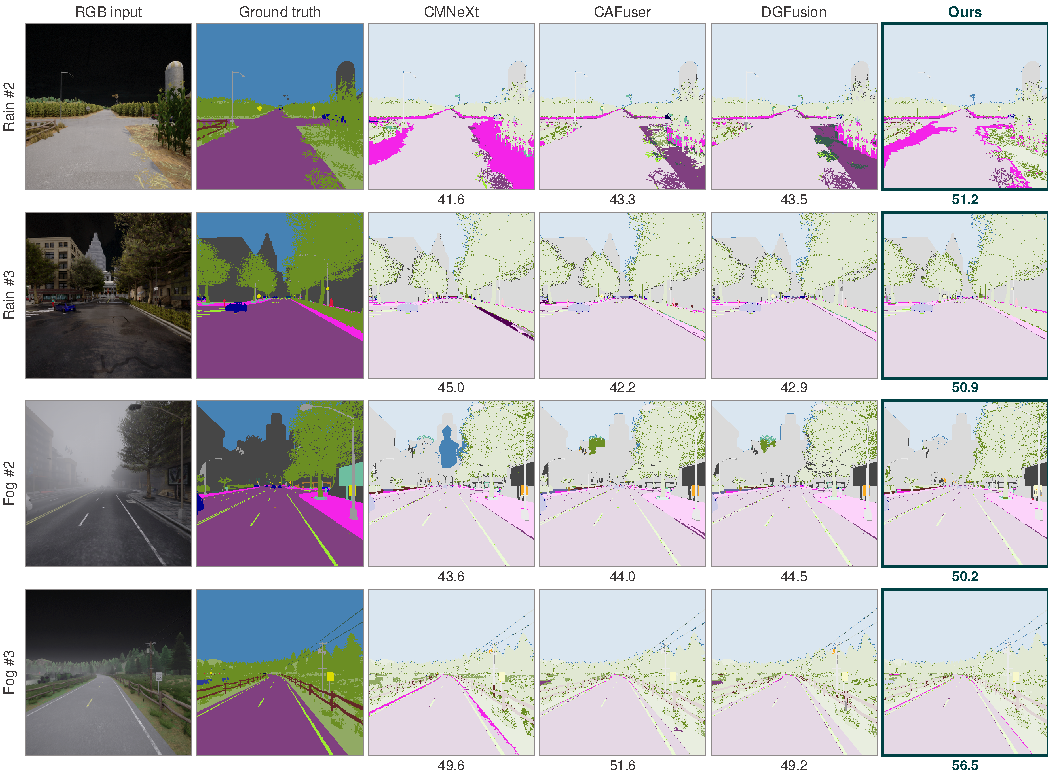
\includegraphics[width=\textwidth]{figures/fig_supp_deliver_2.pdf}\\[3pt]
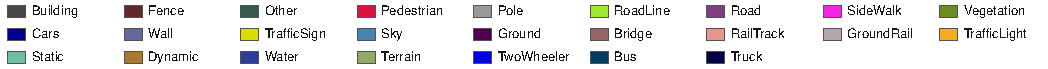
\includegraphics[width=\textwidth]{figures/fig_class_legend_deliver.pdf}
\caption{Additional qualitative results for rain and fog. Display as in Fig.~\ref{fig:supp1}.}
\label{fig:supp2}
\end{figure*}

\begin{figure*}[p]
\centering
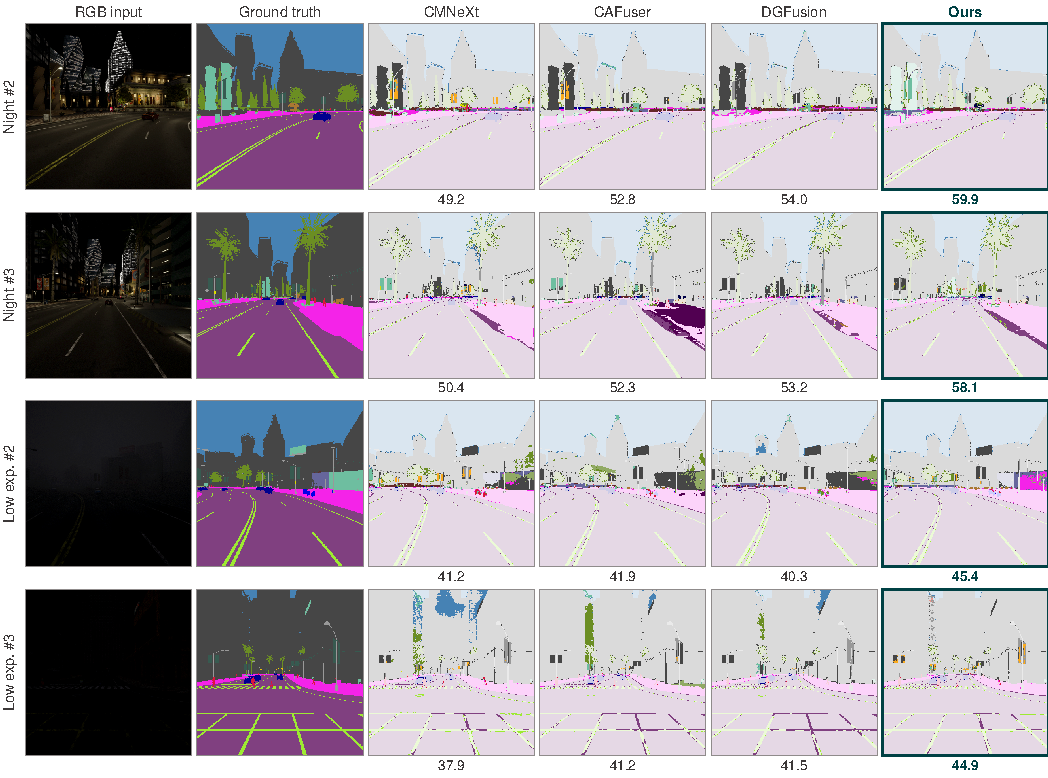
\includegraphics[width=\textwidth]{figures/fig_supp_deliver_3.pdf}\\[3pt]
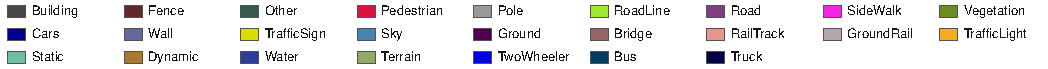
\includegraphics[width=\textwidth]{figures/fig_class_legend_deliver.pdf}
\caption{Additional qualitative results for night and low exposure. Display as in Fig.~\ref{fig:supp1}.}
\label{fig:supp3}
\end{figure*}

\begin{figure*}[p]
\centering
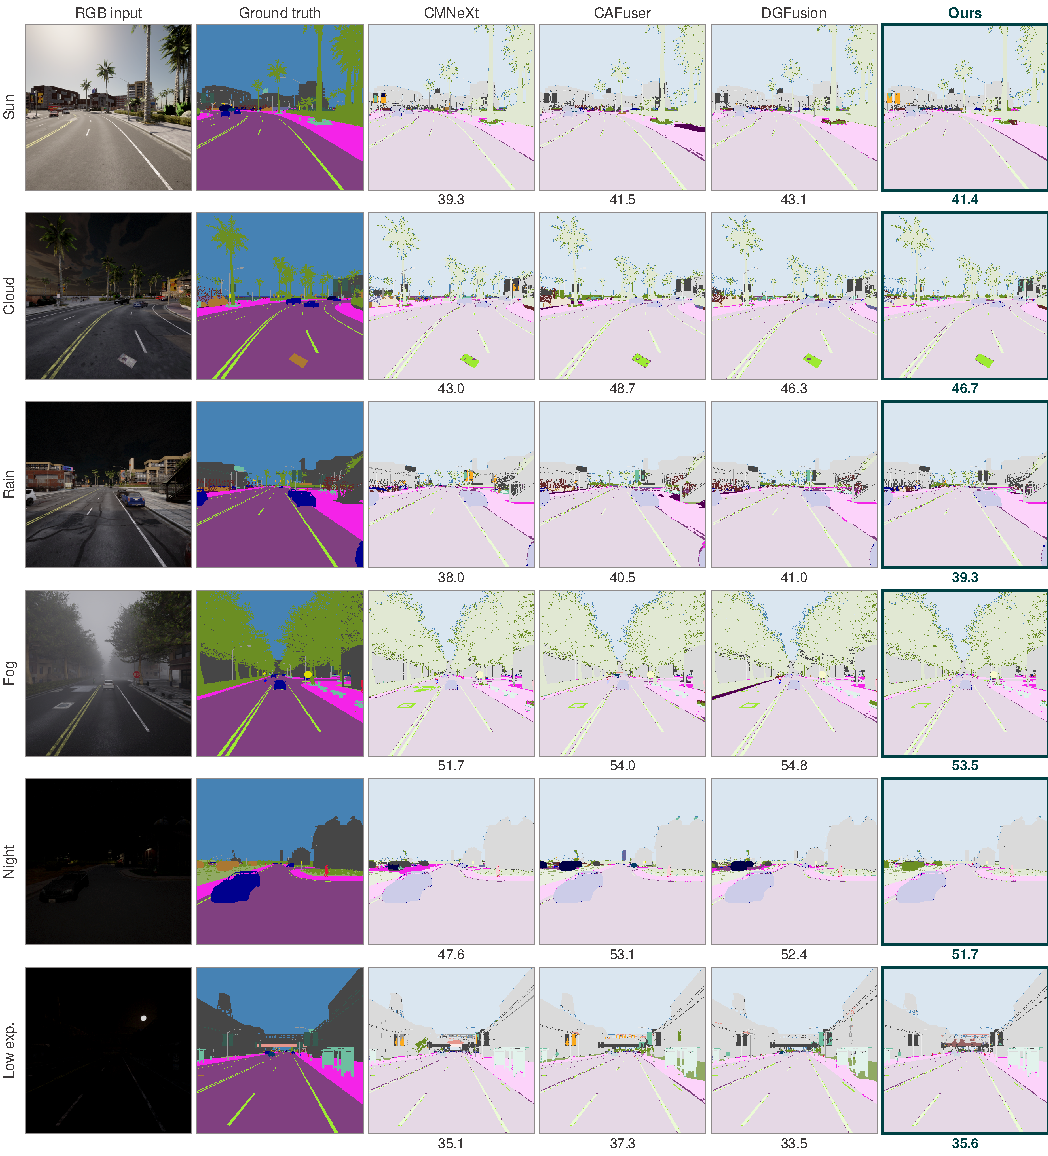
\includegraphics[width=\textwidth]{figures/fig_typical_deliver.pdf}\\[3pt]
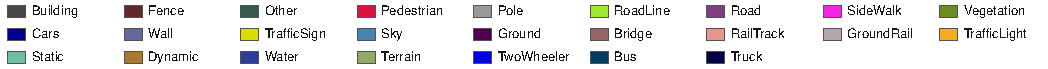
\includegraphics[width=\textwidth]{figures/fig_class_legend_deliver.pdf}
\caption{Typical scenes on the DELIVER test set: for each condition, the image whose per-image mIoU gap between ours and the best other method is closest to the median gap. Display as in Fig.~\ref{fig:supp1}.}
\label{fig:typical}
\end{figure*}

\begin{figure*}[p]
\centering
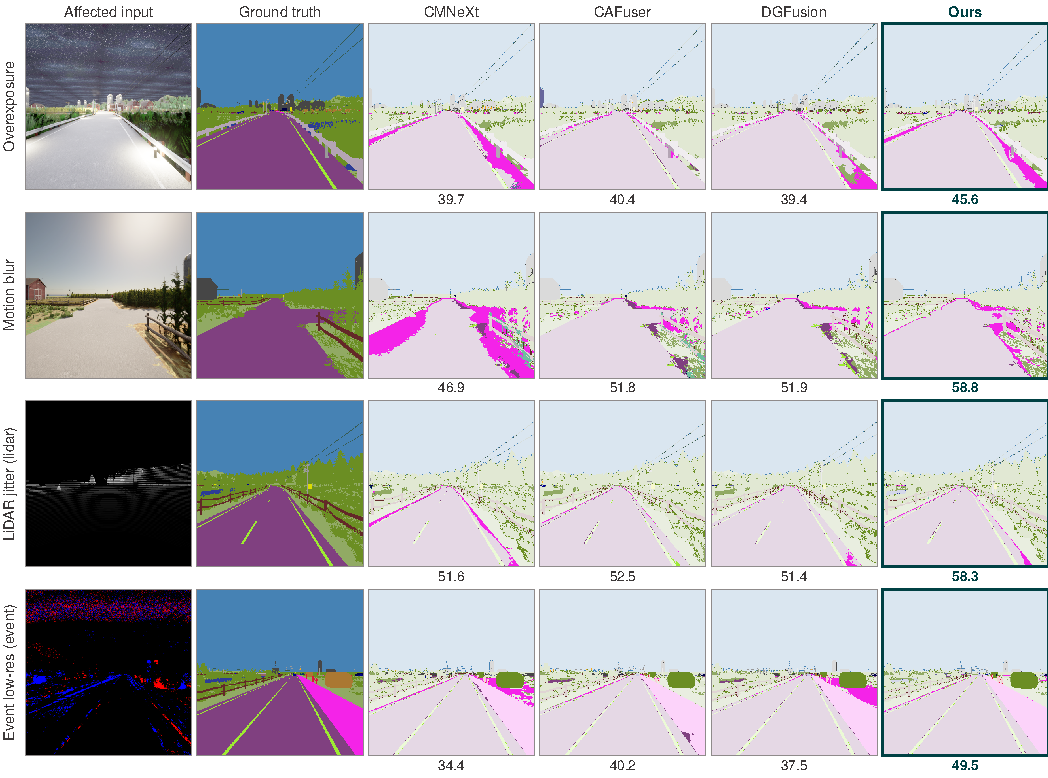
\includegraphics[width=\textwidth]{figures/fig_cases_deliver.pdf}\\[3pt]
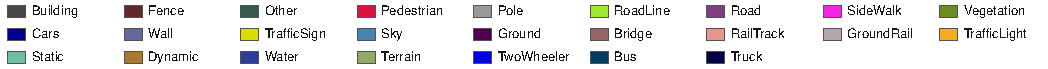
\includegraphics[width=\textwidth]{figures/fig_class_legend_deliver.pdf}
\caption{Qualitative results on DELIVER test sequences with a built-in sensor fault: for each fault, the scene with the largest per-image mIoU gap in favor of ours. The second column shows the affected sensor (RGB for exposure and blur, LiDAR, or event). Display as in Fig.~\ref{fig:supp1}.}
\label{fig:cases}
\end{figure*}

\begin{figure*}[p]
\centering
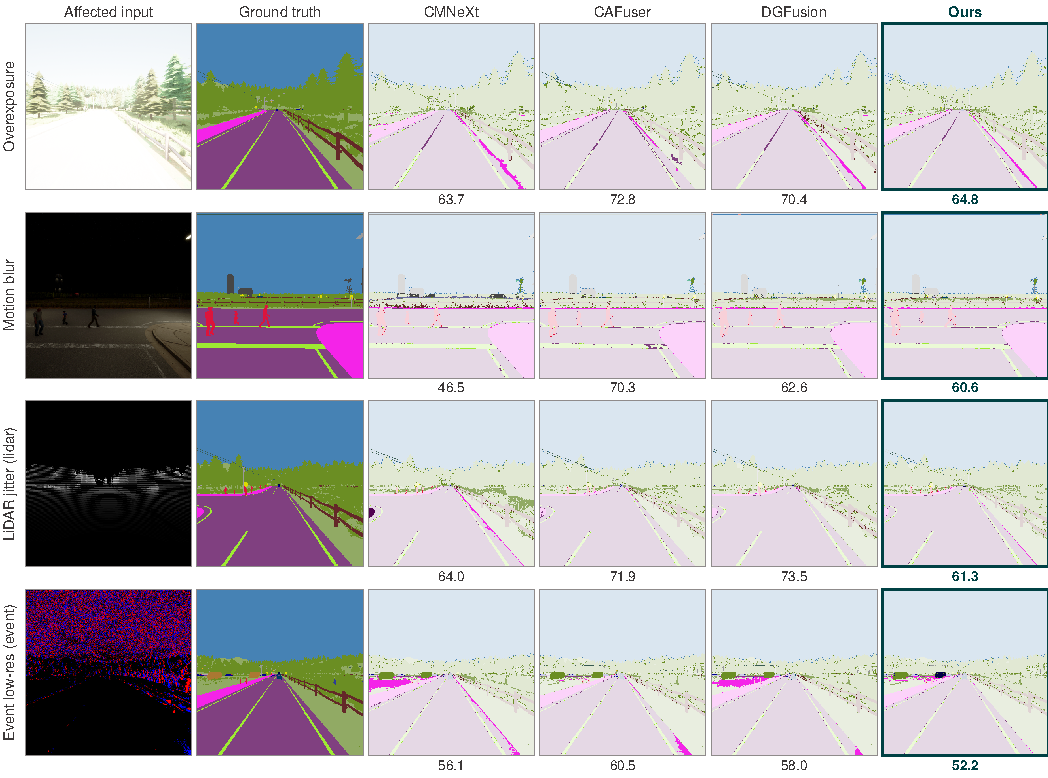
\includegraphics[width=\textwidth]{figures/fig_cases_reverse_deliver.pdf}\\[3pt]
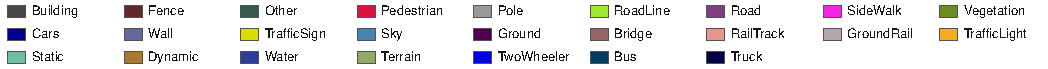
\includegraphics[width=\textwidth]{figures/fig_class_legend_deliver.pdf}
\caption{Failure cases on DELIVER test sequences with a built-in sensor fault: for each fault, the scene where another method most exceeds ours. Display as in Fig.~\ref{fig:cases}.}
\label{fig:cases_reverse}
\end{figure*}

\begin{figure*}[p]
\centering
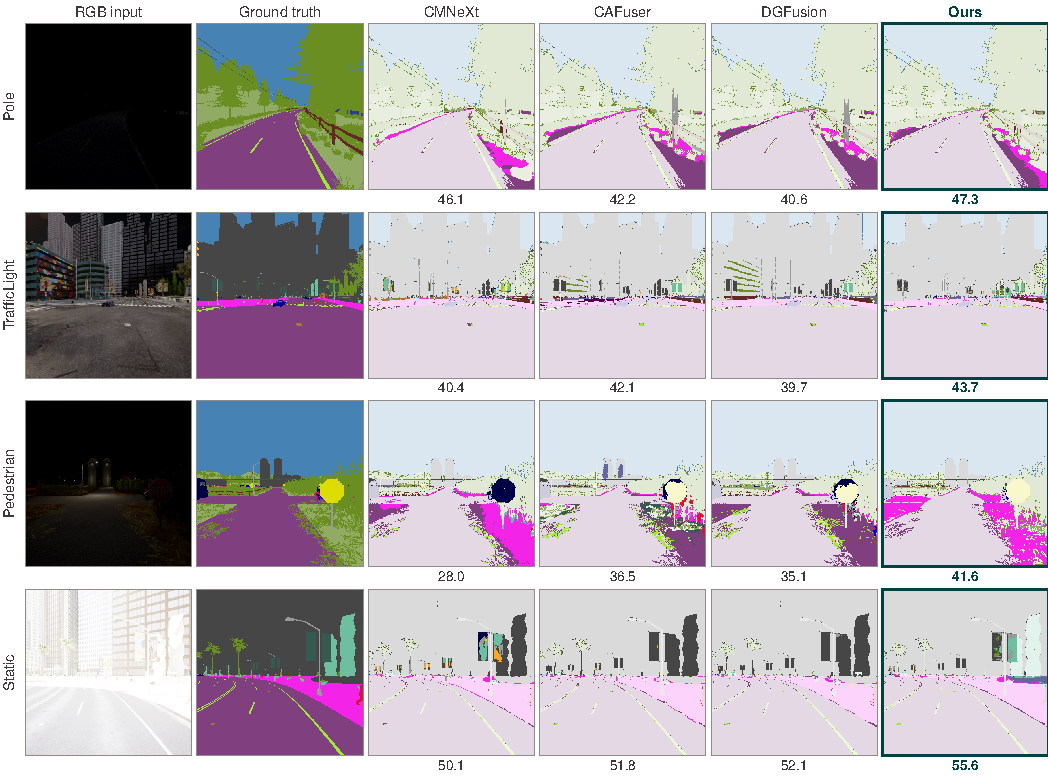
\includegraphics[width=\textwidth]{figures/fig_thin_deliver.pdf}\\[3pt]
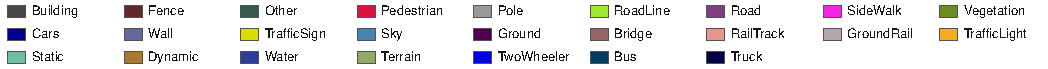
\includegraphics[width=\textwidth]{figures/fig_class_legend_deliver.pdf}
\caption{Thin classes on the DELIVER test set: for each of Pole, TrafficLight, Pedestrian, and Static, the image where the class IoU of ours most exceeds that of the best other method (at least 400 ground-truth pixels of the class). Numbers give per-image mIoU over all classes (\%).}
\label{fig:thin_scenes}
\end{figure*}

\clearpage

% bibliography
\bibliographystyle{IEEEtran}
\bibliography{IEEEabrv,references}

% IEEE Access requires author biographies with photos at the end.
% Bios (user 2026-11-10: write from the RITA paper; it has no bios, so Jemo Maeng's degrees are still to be given).
% Kyoobin Lee: as printed in IEEE Access DOI 10.1109/ACCESS.2026.3684055 and 10.1109/ACCESS.2026.3695573, department renamed to
% AI Graduate School (user 2026-11-10).
\begin{IEEEbiographynophoto}{JEMO MAENG}
(Student Member, IEEE) received the B.S. degree in computer science and technology from Harbin Institute of Technology, China, in 2021, and the M.S. degree from the School of Integrated Technology, Gwangju Institute of Science and Technology (GIST), Republic of Korea, in 2023. He is currently pursuing the Ph.D. degree with the AI Graduate School, GIST, Gwangju, Republic of Korea. His research interests include multi-sensor semantic segmentation, robust perception under sensor failure, and object detection and ranging for autonomous platforms. \todo{photo 1 in $\times$ 1.25 in}
\end{IEEEbiographynophoto}

\begin{IEEEbiographynophoto}{KYOOBIN LEE}
(Member, IEEE) received the B.S., M.S., and Ph.D. degrees in mechanical engineering from Korea Advanced Institute of Science and Technology (KAIST), South Korea, in 2008. From 2008 to 2010, he was a Postdoctoral Scholar with the Center for Neuroscience, KIST. From 2012 to 2017, he was a Principal Researcher with the Samsung Advanced Institute of Technology. Since 2017, he has been a Professor with the AI Graduate School, Gwangju Institute of Science and Technology (GIST). His research interests include vision recognition using deep learning, robot control applications using computer vision, and split learning for neural networks of cloud computing applications. He is an Editor of Korea Robotics Society Review. \todo{photo 1 in $\times$ 1.25 in}
\end{IEEEbiographynophoto}

\EOD
\end{document}
